\documentclass[9pt,a4paper,]{extarticle}

\usepackage{f1000_styles}

\usepackage[pdfborder={0 0 0}]{hyperref}

\usepackage[numbers]{natbib}
\bibliographystyle{unsrtnat}


%% maxwidth is the original width if it is less than linewidth
%% otherwise use linewidth (to make sure the graphics do not exceed the margin)
\makeatletter
\def\maxwidth{ %
  \ifdim\Gin@nat@width>\linewidth
    \linewidth
  \else
    \Gin@nat@width
  \fi
}
\makeatother

\usepackage{color}
\usepackage{fancyvrb}
\newcommand{\VerbBar}{|}
\newcommand{\VERB}{\Verb[commandchars=\\\{\}]}
\DefineVerbatimEnvironment{Highlighting}{Verbatim}{commandchars=\\\{\}}
% Add ',fontsize=\small' for more characters per line
\usepackage{framed}
\definecolor{shadecolor}{RGB}{248,248,248}
\newenvironment{Shaded}{\begin{snugshade}}{\end{snugshade}}
\newcommand{\AlertTok}[1]{\textcolor[rgb]{0.94,0.16,0.16}{#1}}
\newcommand{\AnnotationTok}[1]{\textcolor[rgb]{0.56,0.35,0.01}{\textbf{\textit{#1}}}}
\newcommand{\AttributeTok}[1]{\textcolor[rgb]{0.77,0.63,0.00}{#1}}
\newcommand{\BaseNTok}[1]{\textcolor[rgb]{0.00,0.00,0.81}{#1}}
\newcommand{\BuiltInTok}[1]{#1}
\newcommand{\CharTok}[1]{\textcolor[rgb]{0.31,0.60,0.02}{#1}}
\newcommand{\CommentTok}[1]{\textcolor[rgb]{0.56,0.35,0.01}{\textit{#1}}}
\newcommand{\CommentVarTok}[1]{\textcolor[rgb]{0.56,0.35,0.01}{\textbf{\textit{#1}}}}
\newcommand{\ConstantTok}[1]{\textcolor[rgb]{0.00,0.00,0.00}{#1}}
\newcommand{\ControlFlowTok}[1]{\textcolor[rgb]{0.13,0.29,0.53}{\textbf{#1}}}
\newcommand{\DataTypeTok}[1]{\textcolor[rgb]{0.13,0.29,0.53}{#1}}
\newcommand{\DecValTok}[1]{\textcolor[rgb]{0.00,0.00,0.81}{#1}}
\newcommand{\DocumentationTok}[1]{\textcolor[rgb]{0.56,0.35,0.01}{\textbf{\textit{#1}}}}
\newcommand{\ErrorTok}[1]{\textcolor[rgb]{0.64,0.00,0.00}{\textbf{#1}}}
\newcommand{\ExtensionTok}[1]{#1}
\newcommand{\FloatTok}[1]{\textcolor[rgb]{0.00,0.00,0.81}{#1}}
\newcommand{\FunctionTok}[1]{\textcolor[rgb]{0.00,0.00,0.00}{#1}}
\newcommand{\ImportTok}[1]{#1}
\newcommand{\InformationTok}[1]{\textcolor[rgb]{0.56,0.35,0.01}{\textbf{\textit{#1}}}}
\newcommand{\KeywordTok}[1]{\textcolor[rgb]{0.13,0.29,0.53}{\textbf{#1}}}
\newcommand{\NormalTok}[1]{#1}
\newcommand{\OperatorTok}[1]{\textcolor[rgb]{0.81,0.36,0.00}{\textbf{#1}}}
\newcommand{\OtherTok}[1]{\textcolor[rgb]{0.56,0.35,0.01}{#1}}
\newcommand{\PreprocessorTok}[1]{\textcolor[rgb]{0.56,0.35,0.01}{\textit{#1}}}
\newcommand{\RegionMarkerTok}[1]{#1}
\newcommand{\SpecialCharTok}[1]{\textcolor[rgb]{0.00,0.00,0.00}{#1}}
\newcommand{\SpecialStringTok}[1]{\textcolor[rgb]{0.31,0.60,0.02}{#1}}
\newcommand{\StringTok}[1]{\textcolor[rgb]{0.31,0.60,0.02}{#1}}
\newcommand{\VariableTok}[1]{\textcolor[rgb]{0.00,0.00,0.00}{#1}}
\newcommand{\VerbatimStringTok}[1]{\textcolor[rgb]{0.31,0.60,0.02}{#1}}
\newcommand{\WarningTok}[1]{\textcolor[rgb]{0.56,0.35,0.01}{\textbf{\textit{#1}}}}

% disable code chunks background
%\renewenvironment{Shaded}{}{}

% disable section numbers
\setcounter{secnumdepth}{0}

%% added by MLS, this is not in the F1000 style by default %%

\hypersetup{unicode=true,
            pdftitle={BASiCS workflow: a step-by-step analysis of expression variability using single cell RNA sequencing data},
            pdfkeywords={Single-cell RNA sequencing, expression variability, transcriptional noise, differential expression testing},
            colorlinks=true,
            linkcolor=Maroon,
            citecolor=Blue,
            urlcolor=Orange,
            breaklinks=true}

%% End added by MLS %%

\setlength{\parindent}{0pt}
\setlength{\parskip}{6pt plus 2pt minus 1pt}



\begin{document}
\pagestyle{front}

\title{BASiCS workflow: a step-by-step analysis of expression variability using single cell RNA sequencing data}

\author[1]{Alan O'Callaghan\thanks{\ttfamily a.b.o'callaghan@sms.ed.ac.uk}}
\author[2]{Nils Eling}
\author[3,4]{John C. Marioni}
\author[1,5]{Catalina A. Vallejos\thanks{\ttfamily catalina.vallejos@igmm.ed.ac.uk}}
\affil[1]{MRC Human Genetics Unit, Institute of Genetics \& Molecular Medicine, University of Edinburgh, Western General Hospital, Crewe Road, Edinburgh, EH4 2XU, UK}
\affil[2]{Department of Quantitative Biomedicine, University of Zurich, Winterthurerstrasse 190, CH-8057, Zurich, Switzerland}
\affil[3]{European Molecular Biology Laboratory, European Bioinformatics Institute, Wellcome Trust Genome Campus, Hinxton, Cambridge CB10 1SD, UK}
\affil[4]{Cancer Research UK Cambridge Institute, University of Cambridge, Li Ka Shing Centre, Cambridge, CB2 0RE, UK}
\affil[5]{The Alan Turing Institute, British Library, 96 Euston Road, London, NW1 2DB, UK}

\maketitle
\thispagestyle{front}

\begin{abstract}
Cell-to-cell gene expression variability is an inherent feature of complex
biological systems, such as immunity and development. Single-cell RNA
sequencing is a powerful tool to quantify this heterogeneity, but it is prone
to strong technical noise. In this article, we describe a step-by-step
computational workflow that uses the BASiCS Bioconductor package to robustly
quantify expression variability within and between known groups of cells (such
as experimental conditions or cell types). BASiCS uses an integrated framework
for data normalisation, technical noise quantification and downstream
analyses, whilst propagating statistical uncertainty across these steps.
Within a single seemingly homogeneous cell population, BASiCS can identify
highly variable genes that exhibit strong heterogeneity as well as lowly
variable genes with stable expression. BASiCS also uses a probabilistic
decision rule to identify changes in expression variability between cell
populations, whilst avoiding confounding effects related to differences in
technical noise or in overall abundance. Using a publicly available
dataset, we guide users through a complete pipeline that includes
preliminary steps for quality control, as well as data exploration
using the scater and scran Bioconductor packages. The workflow is accompanied
by a Docker image that ensures the reproducibility of our results.
\end{abstract}

\section*{Keywords}
Single-cell RNA sequencing, expression variability, transcriptional noise, differential expression testing


\clearpage
\pagestyle{main}

\hypertarget{introduction}{%
\section{Introduction}\label{introduction}}

Single-cell RNA-sequencing (scRNA-seq) enables the study of genome-wide
transcriptional heterogeneity in cell populations that is not
captured by bulk experiments \citep{Stegle2015, Prakadan2017, Patange2018}.
On the broadest level, this heterogeneity can reflect the presence of distinct
cell subtypes or states.
Alternatively, it can be due to gradual changes along biological processes,
such as development and differentiation.
Several clustering and pseudotime inference methods have been developed to
characterise these types of heterogeneity \citep{Kiselev2019, Saelens2019}.
However, there is a limited availability of computational tools tailored
to study more subtle variability within seemingly homogeneous cell populations.
This variability can reflect deterministic or stochastic events that regulate
gene expression and, among others, has been reported to increase prior to cell
fate decisions \citep{Mojtahedi2016} as well as during ageing \citep{Martinez-jimenez2017}.

Stochastic variability within a seemingly homogeneous cell population --- often
referred to as transcriptional \emph{noise} --- can arise from intrinsic and
extrinsic sources \citep{Elowitz2002, Eling2019}.
Extrinsic noise refers to stochastic fluctuations induced by
different dynamic cellular states (e.g.~cell cycle, metabolism,
intra/inter-cellular signalling) \citep{Zopf2013, Iwamoto2016, Kiviet2014}.
In contrast, intrinsic noise arises from stochastic effects on biochemical
processes such as transcription and translation \citep{Elowitz2002}.
Intrinsic noise can be modulated by genetic and epigenetic modifications (such
as mutations, histone modifications, CpG island length and nucleosome
positioning) \citep{Eberwine2015, Faure2017, Morgan2018} and usually occurs
at the gene level \citep{Elowitz2002}.
Cell-to-cell gene expression variability estimates derived from scRNA-seq data
capture a combination of these effects, as well as deterministic regulatory
mechanisms \citep{Eling2019}.
Moreover, these variability estimates can also be inflated by the technical
noise that is typically observed in scRNA-seq data \citep{Brennecke2013}.

Different strategies have been incorporated into scRNA-seq protocols to control
or attenuate technical noise.
For example, external RNA spike-in molecules (such as the set introduced by the
External RNA Controls Consortium, ERCC \citep{Rna2005}) can be added to each cell's
lysate in a (theoretically) known fixed quantity.
Spike-ins can assist quality control steps \citep{McCarthy2017}, data normalisation
\citep{Vallejos2017} and can be used to infer technical noise \citep{Brennecke2013}.
Another strategy is to tag individual cDNA molecules using unique molecular
identifiers (UMIs) before PCR amplification \citep{Islam2014}.
Reads that contain the same UMI can be collapsed into a single molecule count,
attenuating technical variability associated to cell-to-cell differences
in amplification and sequencing depth (these technical biases are not fully
removed unless sequencing to saturation \citep{Vallejos2017}).
However, despite the benefits associated to the use of spike-ins and UMIs,
these are not available for all scRNA-seq protocols \citep{Haque2017}.

The Bioconductor package \emph{\href{https://bioconductor.org/packages/3.11/BASiCS}{BASiCS}} implements a Bayesian
hierarchical framework that accounts for both technical and biological sources
of noise in scRNA-seq datasets \citep{Vallejos2015, Vallejos2016, Eling2017}.
\emph{\href{https://bioconductor.org/packages/3.11/BASiCS}{BASiCS}} jointly performs data normalisation, technical noise
quantification and downstream analyses, whilst propagating statistical
uncertainty across these steps.
These features are implemented within a probabilistic model that builds upon a
negative binomial framework, a widely used distribution in the context of bulk
and scRNA-seq experiments \citep{Svensson2020, Townes2020, Townes2019}.
Critically, \emph{\href{https://bioconductor.org/packages/3.11/BASiCS}{BASiCS}} enables the quantification of transcriptional
variability within a population of cells, while accounting for the overall
mean-variance relationship that typically arises in scRNA-seq data \citep{Eling2018}.
Furthermore, when available, \emph{\href{https://bioconductor.org/packages/3.11/BASiCS}{BASiCS}} can also leverage extrinsic
spike-in molecules to aid data normalisation.

This article complements existing scRNA-seq workflows based on the Bioconductor
ecosystem (e.g.~\citep{Lun2016, Kim2019}), providing a detailed framework for
transcriptional variability analyses using \emph{\href{https://bioconductor.org/packages/3.11/BASiCS}{BASiCS}}.
We describe a step-by-step workflow that uses \emph{\href{https://bioconductor.org/packages/3.11/scater}{scater}}
\citep{McCarthy2017} and \emph{\href{https://bioconductor.org/packages/3.11/scran}{scran}} \citep{Lun2016} to perform quality control
(QC) as well as initial exploratory analyses.
Our analysis pipeline includes practical guidance to assess the convergence of
the Markov Chain Monte Carlo (MCMC) algorithm that is used to infer model
parameters in \emph{\href{https://bioconductor.org/packages/3.11/BASiCS}{BASiCS}}, as well as recommendations to interpret
and post-process the model outputs.
Finally, through a case study in the context of immune cells, we illustrate
how \emph{\href{https://bioconductor.org/packages/3.11/BASiCS}{BASiCS}} can be used to identify highly and lowly variable
genes within a cell population, as well as to compare expression profiles
between experimental conditions or cell types.

All source code used to generate the results presented in this article is
available \href{https://github.com/VallejosGroup/BASiCSWorkflow}{on Github}.
To ensure the
reproducibility of this workflow, the analysis environment and all software
dependencies are provided as a Docker image \citep{Boettiger2015}. The image
can be obtained from
\href{https://hub.docker.com/repository/docker/alanocallaghan/bocker}{Docker Hub}.

\hypertarget{methods}{%
\section{Methods}\label{methods}}

This step-by-step scRNA-seq workflow is primarily based on the Bioconductor
package ecosystem \citep{Amezquita2019}.
A graphical overview is provided in Figure \ref{fig:overview}
and its main components are described below.

\begin{figure}

{\centering 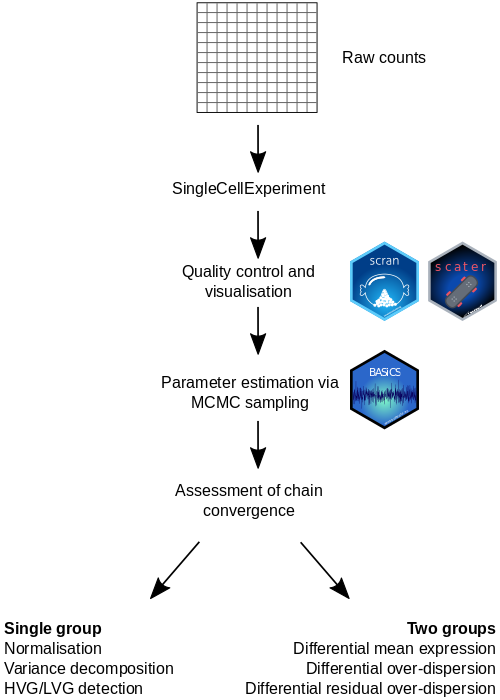
\includegraphics[width=2.5in,height=3.5in]{figure/Overview} 

}

\caption{Graphical overview for the scRNA-seq analysis workflow described in this manuscript. Starting from a matrix of expression counts, we use the scater and scran Bioconductor packages to perform QC and initial exploratory analyses. To robustly quantify transcriptional heterogeneity within seemingly homogeneous cell populations, we apply the BASiCS Bioconductor package and  illustrate how BASiCS can be used to analyse a single or multiple pre-specified groups of cells.}\label{fig:overview}
\end{figure}

\hypertarget{input-data}{%
\subsubsection{Input data}\label{input-data}}

\begin{Shaded}
\begin{Highlighting}[]
\KeywordTok{library}\NormalTok{(}\StringTok{"SingleCellExperiment"}\NormalTok{)}
\end{Highlighting}
\end{Shaded}

We use \emph{\href{https://bioconductor.org/packages/3.11/SingleCellExperiment}{SingleCellExperiment}} to convert an input
matrix of raw read-counts (molecule counts for UMI-based protocols) into a
\texttt{SingleCellExperiment} object that can also store its associated
metadata, such as gene- and cell-specific information.
Moreover, when available, the same object can also store read-counts for
spike-in molecules (see \texttt{?altExp}).
A major advantage of using a \texttt{SingleCellExperiment} object as the input for
scRNA-seq analyses is the interoperability across a large number of
Bioconductor packages \citep{Amezquita2019}.

\hypertarget{qc-and-exploratory-data-analysis}{%
\subsection{QC and exploratory data analysis}\label{qc-and-exploratory-data-analysis}}

\begin{Shaded}
\begin{Highlighting}[]
\KeywordTok{library}\NormalTok{(}\StringTok{"scater"}\NormalTok{)}
\KeywordTok{library}\NormalTok{(}\StringTok{"scran"}\NormalTok{)}
\end{Highlighting}
\end{Shaded}

An critical step in scRNA-seq analyses is QC, removing low quality samples that
may distort downstream analyses.
In this step, we use QC diagnostics to identify and remove samples that
correspond to broken cells, that are empty, or that contain multiple cells
\citep{Ilicic2016}. We also typically remove lowly expressed genes that represent
less reliable information.
The \href{https://osca.bioconductor.org/}{\emph{OSCA}} online book provides an extensive
overview on important aspects of how to perform QC of scRNA-seq data, including
exploratory analyses \citep{Amezquita2019}.

Here, we use the \emph{\href{https://bioconductor.org/packages/3.11/scater}{scater}} package \citep{McCarthy2017} to calculate
QC metrics for each cell (e.g.~total read-count) and gene (e.g.~percentage of
zeroes across all cells), respectively.
Moreover, we use the visualisation tools implemented in \emph{\href{https://bioconductor.org/packages/3.11/scater}{scater}} to
explore the input dataset and its associated QC diagnostic metrics.
For further exploratory data analysis we use the \emph{\href{https://bioconductor.org/packages/3.11/scran}{scran}} package
\citep{Lun2016}.
The latter can perform \emph{global scaling} normalisation, calculating
cell-specific scaling factors that capture global differences in read-counts
across cells (e.g.~due to sequencing depth and PCR amplification)
\citep{Lun2016pooling}.
To quantify transcriptional variability, \emph{\href{https://bioconductor.org/packages/3.11/scran}{scran}} can be used to
infer an overall trend between mean expression and the squared coefficent of
variation (CV\textsuperscript{2}) for each gene.
To derive variability estimates that are not confounded by this overall trend,
\emph{\href{https://bioconductor.org/packages/3.11/scran}{scran}} also defines gene-specific DM (distance to the mean)
estimates as the distance between CV\(^2\) and a rolling median along the range
of mean expression values \citep{Kolodziejczyk2015cell}.
DM estimates enable exploratory analyses of cell-to-cell gene expression
variability, but a measure of statistical uncertainty is not readily available
for these estimates.
As such, gene-specific downstream inference (such as differential variability
testing) is precluded.

\hypertarget{basics---bayesian-analysis-of-single-cell-sequencing-data}{%
\subsection{BASiCS - Bayesian Analysis of Single Cell Sequencing data}\label{basics---bayesian-analysis-of-single-cell-sequencing-data}}

\begin{Shaded}
\begin{Highlighting}[]
\KeywordTok{library}\NormalTok{(}\StringTok{"BASiCS"}\NormalTok{)}
\end{Highlighting}
\end{Shaded}

The \emph{\href{https://bioconductor.org/packages/3.11/BASiCS}{BASiCS}} package uses a Bayesian hierarchical framework
that borrows information across all genes and cells to robustly quantify
transcriptional variability \citep{Vallejos2015BASiCS}.
Similar to the approach adopted in \emph{\href{https://bioconductor.org/packages/3.11/scran}{scran}}, \emph{\href{https://bioconductor.org/packages/3.11/BASiCS}{BASiCS}}
infers cell-specific global scaling normalisation parameters.
However, instead of inferring these as a pre-processing step,
\emph{\href{https://bioconductor.org/packages/3.11/BASiCS}{BASiCS}} uses an integrated approach wherein data normalisation
and downstream analyses are performed simultaneously, thereby propagating
statistical uncertainty.
To quantify technical noise, the original implementation of
\emph{\href{https://bioconductor.org/packages/3.11/BASiCS}{BASiCS}} uses information from extrinsic spike-in molecules as
control features, but the model has been extended to address situations wherein
spike-ins are not available \citep{Eling2018}.

\emph{\href{https://bioconductor.org/packages/3.11/BASiCS}{BASiCS}} summarises the expression pattern for each gene through
gene-specific \emph{mean} and \emph{over-dispersion} parameters.
Mean parameters \(\mu_i\) quantify the overall expression for each gene \(i\)
across the cell population under study.
In contrast, \(\delta_i\) captures the excess of variability that is observed with
respect to what would be expected in a homogeneous cell population, beyond
technical noise.
\emph{\href{https://bioconductor.org/packages/3.11/BASiCS}{BASiCS}} uses \(\delta_i\) as a proxy to quantify transcriptional
variability.
To account for the strong relationship that is typically observed
between gene-specific mean expression and over-dispersion estimates,
Eling \emph{et al.} \citep{Eling2018} introduced a joint prior specification for
these parameters.
This joint prior formulation has been observed to improve posterior inference
when the data is less informative (e.g.~small sample size, lowly expressed
genes), borroring information across all genes to infer an overall trend that
captures the relationship between mean and over-dispersion.
The trend is then used to derive gene-specific \emph{residual over-dispersion}
parameters \(\epsilon_i\) that are not confounded by mean expression.
Similar to DM values implemented in \emph{\href{https://bioconductor.org/packages/3.11/scran}{scran}}, these are defined as
deviations with respect to the overall trend.

Within a population of cells, \emph{\href{https://bioconductor.org/packages/3.11/BASiCS}{BASiCS}} decomposes the total
observed variability in expression measurements into technical and biological
components \citep{Vallejos2015}.
This enables the identification of \emph{highly variable genes} (HVGs) that capture
the major sources of heterogeneity within the analysed cells \citep{Brennecke2013}.
HVG detection is often used as feature selection, to identify the input
set of genes for subsequent analyses.
\emph{\href{https://bioconductor.org/packages/3.11/BASiCS}{BASiCS}} can also highlight \emph{lowly variable genes} (LVGs) that
exhibit stable expression across the population of cells.
These may relate to essential cellular functions and can assist the development
of new data normalisation or integration strategies \citep{Lin2019}.

\emph{\href{https://bioconductor.org/packages/3.11/BASiCS}{BASiCS}} also provides a probabilistic decision rule to
perform differential expression analyses between two (or more) pre-specified
groups of cells \citep{Vallejos2016, Eling2018}.
While several differential expression tools have been proposed for scRNA-seq
data (e.g.~\citep{Kharchenko2014, Finak2015}), some evidence suggests that
these do not generally outperform popular bulk RNA-seq tools \citep{Soneson2018}.
Moreover, most of these methods are only designed to uncover changes in overall
expression, ignoring the more complex patterns that can arise at the single cell
level \citep{Lahnemann2020}.
Instead, \emph{\href{https://bioconductor.org/packages/3.11/BASiCS}{BASiCS}} embraces the high granularity of scRNA-seq data,
uncovering changes in cell-to-cell expression variability that are not
confounded by differences in technical noise or in overall expression.

\hypertarget{Tcells}{%
\section{\texorpdfstring{Case study: analysis of naive CD4\textsuperscript{+} T cells}{Case study: analysis of naive CD4+ T cells}}\label{Tcells}}

As a case study, we use scRNA-seq data generated for CD4\textsuperscript{+} T cells
using the C1 Single-Cell Auto Prep System (Fluidigm\textsuperscript{®}).
Martinez-Jimenez \emph{et al.} profiled naive (hereafter also referred to as
unstimulated) and activated (3 hours using \emph{in vitro} antibody stimulation)
CD4\textsuperscript{+} T cells from young and old animals across two mouse strains to study
changes in expression variability during ageing and upon immune activation
\citep{Martinez-jimenez2017}.
They extracted naive or effector memory CD4\textsuperscript{+} T cells from spleens of young or
old animals, obtaining purified populations using either magnetic-activated cell
sorting (MACS) or fluorescence activated cell sorting (FACS).
External ERCC spike-in RNA \citep{Rna2005} was added to aid the quantification of
technical variability across all cells and all experiments were performed in
replicates (hereafter also referred to as batches).

\hypertarget{downloading-the-data}{%
\subsection{Downloading the data}\label{downloading-the-data}}

The matrix with raw read counts can be obtained from ArrayExpress under the
accession number
\href{https://www.ebi.ac.uk/arrayexpress/experiments/E-MTAB-4888/}{E-MTAB-4888}.
In the matrix, column names contain library identifiers and row names
display gene Ensembl identifiers.

\begin{Shaded}
\begin{Highlighting}[]
\ControlFlowTok{if}\NormalTok{ (}\OperatorTok{!}\KeywordTok{file.exists}\NormalTok{(}\StringTok{"downloads/"}\NormalTok{))}
  \KeywordTok{dir.create}\NormalTok{(}\StringTok{"downloads"}\NormalTok{, }\DataTypeTok{showWarnings =} \OtherTok{FALSE}\NormalTok{)}
\ControlFlowTok{if}\NormalTok{ (}\OperatorTok{!}\KeywordTok{file.exists}\NormalTok{(}\StringTok{"downloads/raw_data.txt"}\NormalTok{)) \{}
\NormalTok{  website <-}\StringTok{ "https://www.ebi.ac.uk/arrayexpress/files/E-MTAB-4888/"}
\NormalTok{  file <-}\StringTok{ "E-MTAB-4888.processed.1.zip"}
  \KeywordTok{download.file}\NormalTok{(}
    \KeywordTok{paste0}\NormalTok{(website, file),}
    \DataTypeTok{destfile =} \StringTok{"downloads/raw_data.txt.zip"}
\NormalTok{  )}
  \KeywordTok{unzip}\NormalTok{(}\StringTok{"downloads/raw_data.txt.zip"}\NormalTok{, }\DataTypeTok{exdir =} \StringTok{"downloads"}\NormalTok{)}
  \KeywordTok{file.remove}\NormalTok{(}\StringTok{"downloads/raw_data.txt.zip"}\NormalTok{)}
\NormalTok{\}}

\NormalTok{CD4_raw <-}\StringTok{ }\KeywordTok{read.table}\NormalTok{(}\StringTok{"downloads/raw_data.txt"}\NormalTok{, }\DataTypeTok{header =} \OtherTok{TRUE}\NormalTok{, }\DataTypeTok{sep =} \StringTok{"}\CharTok{\textbackslash{}t}\StringTok{"}\NormalTok{)}
\NormalTok{CD4_raw <-}\StringTok{ }\KeywordTok{as.matrix}\NormalTok{(CD4_raw)}
\end{Highlighting}
\end{Shaded}

The input matrix contains data for 1,513
cells and 31,181
genes (including 92 ERCC spike-ins).
Information about experimental conditions and other metadata is available
under the same accession number.

\begin{Shaded}
\begin{Highlighting}[]
\ControlFlowTok{if}\NormalTok{ (}\OperatorTok{!}\KeywordTok{file.exists}\NormalTok{(}\StringTok{"downloads/metadata_file.txt"}\NormalTok{)) \{}
\NormalTok{  website <-}\StringTok{ "https://www.ebi.ac.uk/arrayexpress/files/E-MTAB-4888"}
\NormalTok{  file <-}\StringTok{ "E-MTAB-4888.additional.1.zip"}
  \KeywordTok{download.file}\NormalTok{(}
    \KeywordTok{paste0}\NormalTok{(website, file),}
    \DataTypeTok{destfile =} \StringTok{"downloads/metadata.txt.zip"}
\NormalTok{  )}
  \KeywordTok{unzip}\NormalTok{(}\StringTok{"downloads/metadata.txt.zip"}\NormalTok{, }\DataTypeTok{exdir =} \StringTok{"downloads"}\NormalTok{)}
  \KeywordTok{file.remove}\NormalTok{(}\StringTok{"downloads/metadata.txt.zip"}\NormalTok{)}
\NormalTok{\}}

\NormalTok{CD4_metadata <-}\StringTok{ }\KeywordTok{read.table}\NormalTok{(}
  \StringTok{"downloads/metadata_file.txt"}\NormalTok{,}
  \DataTypeTok{header =} \OtherTok{TRUE}\NormalTok{,}
  \DataTypeTok{sep =} \StringTok{"}\CharTok{\textbackslash{}t}\StringTok{"}
\NormalTok{)}

\CommentTok{# Save sample identifiers as rownames}
\KeywordTok{rownames}\NormalTok{(CD4_metadata) <-}\StringTok{ }\NormalTok{CD4_metadata}\OperatorTok{$}\NormalTok{X}
\end{Highlighting}
\end{Shaded}

The columns in the metadata file contain library identifiers (\texttt{X}), strain
information (\texttt{Strain}; \emph{Mus musculus castaneus} or \emph{Mus musculus domesticus}),
the age of the animals (\texttt{Age}; young or old), stimulation state of the cells
(\texttt{Stimulus}; naive or activated), batch information (\texttt{Individuals}; associated
to different mice), and cell type information (\texttt{Celltype}; via FACS or MACS
purification).

Here, we convert the data and metadata described above into a
\texttt{SingleCellExperiment} object.
For this purpose, we first separate the input matrix of expression counts into
two matrices associated to intrinsic genes and external spike-ins, respectively.
Within the \texttt{SingleCellExperiment} object, the latter is stored separately
as an \emph{alternative experiment} (see \texttt{?altExp}).

\begin{Shaded}
\begin{Highlighting}[]
\CommentTok{# Separate intrinsic from ERCC counts}
\NormalTok{bio_counts <-}\StringTok{ }\NormalTok{CD4_raw[}\OperatorTok{!}\KeywordTok{grepl}\NormalTok{(}\StringTok{"ERCC"}\NormalTok{, }\KeywordTok{rownames}\NormalTok{(CD4_raw)), ]}
\NormalTok{spike_counts <-}\StringTok{ }\NormalTok{CD4_raw[}\KeywordTok{grepl}\NormalTok{(}\StringTok{"ERCC"}\NormalTok{, }\KeywordTok{rownames}\NormalTok{(CD4_raw)), ]}
\CommentTok{# Generate the SingleCellExperiment object}
\NormalTok{sce_CD4_all <-}\StringTok{ }\KeywordTok{SingleCellExperiment}\NormalTok{(}
  \DataTypeTok{assays =} \KeywordTok{list}\NormalTok{(}\DataTypeTok{counts =} \KeywordTok{as.matrix}\NormalTok{(bio_counts)),}
  \DataTypeTok{colData =}\NormalTok{ CD4_metadata[}\KeywordTok{colnames}\NormalTok{(CD4_raw), ]}
\NormalTok{)}
\CommentTok{# Add read-counts for spike-ins as an alternative experiment}
\KeywordTok{altExp}\NormalTok{(sce_CD4_all, }\StringTok{"spike-ins"}\NormalTok{) <-}\StringTok{ }\KeywordTok{SummarizedExperiment}\NormalTok{(}
  \DataTypeTok{assays =} \KeywordTok{list}\NormalTok{(}\DataTypeTok{counts =}\NormalTok{ spike_counts)}
\NormalTok{)}
\end{Highlighting}
\end{Shaded}

Hereafter, our analysis focuses on naive and activated CD4\textsuperscript{+} T cells obtained
from young \emph{Mus musculus domesticus} animals, purified using MACS-based cell sorting.
Here, we extract these
146 samples.

\begin{Shaded}
\begin{Highlighting}[]
\NormalTok{ind_select <-}\StringTok{ }\NormalTok{sce_CD4_all}\OperatorTok{$}\NormalTok{Strain }\OperatorTok{==}\StringTok{ "Mus musculus domesticus"} \OperatorTok{&}
\StringTok{  }\NormalTok{sce_CD4_all}\OperatorTok{$}\NormalTok{Age }\OperatorTok{==}\StringTok{ "Young"} \OperatorTok{&}
\StringTok{  }\NormalTok{sce_CD4_all}\OperatorTok{$}\NormalTok{Celltype }\OperatorTok{==}\StringTok{ "MACS-purified Naive"}
\NormalTok{sce_naive_active <-}\StringTok{ }\NormalTok{sce_CD4_all[, ind_select]}
\NormalTok{sce_naive_active}
\end{Highlighting}
\end{Shaded}

\begin{verbatim}
## class: SingleCellExperiment 
## dim: 31089 146 
## metadata(0):
## assays(1): counts
## rownames(31089): ENSMUSG00000000001 ENSMUSG00000000003 ...
##   ENSMUSG00000106668 ENSMUSG00000106670
## rowData names(0):
## colnames(146): do6113 do6118 ... do6493 do6495
## colData names(6): X Strain ... Individuals Celltype
## reducedDimNames(0):
## altExpNames(1): spike-ins
\end{verbatim}

\hypertarget{annotation}{%
\subsection{Annotation}\label{annotation}}

Input read counts were annotated using Ensembl gene identifiers.
In order to facilitate the visualisation and interpretation of results, it is
often useful to generate a mapping from Ensembl gene IDs to gene symbols using
the BioMart software suite (\url{http://www.biomart.org})
via the Bioconductor package, \emph{\href{https://bioconductor.org/packages/3.11/biomaRt}{biomaRt}} \citep{Durinck2009}.
These packages can also be used to obtain gene-pathways mappings and other
information such as gene length, useful for performing functional analysis
of the gene sets identified in downstream analyses.

\begin{Shaded}
\begin{Highlighting}[]
\ControlFlowTok{if}\NormalTok{(}\OperatorTok{!}\KeywordTok{file.exists}\NormalTok{(}\StringTok{"rds/"}\NormalTok{))}
  \KeywordTok{dir.create}\NormalTok{(}\StringTok{"rds"}\NormalTok{, }\DataTypeTok{showWarnings =} \OtherTok{FALSE}\NormalTok{)}

\KeywordTok{library}\NormalTok{(biomaRt)}

\ControlFlowTok{if}\NormalTok{ (}\OperatorTok{!}\KeywordTok{file.exists}\NormalTok{(}\StringTok{"rds/genenames.rds"}\NormalTok{)) \{}
  \CommentTok{# Initialize mart and dataset}
\NormalTok{  ensembl <-}\StringTok{ }\KeywordTok{useMart}\NormalTok{(}
    \DataTypeTok{biomart =} \StringTok{"ensembl"}\NormalTok{,}
    \DataTypeTok{dataset =} \StringTok{"mmusculus_gene_ensembl"}
\NormalTok{  )}
  
  \CommentTok{# Select gene ID and gene name}
\NormalTok{  genenames <-}\StringTok{ }\KeywordTok{getBM}\NormalTok{(}
    \DataTypeTok{attributes =} \KeywordTok{c}\NormalTok{(}\StringTok{"ensembl_gene_id"}\NormalTok{, }\StringTok{"external_gene_name"}\NormalTok{),}
    \DataTypeTok{mart =}\NormalTok{ ensembl}
\NormalTok{  )}

  \KeywordTok{rownames}\NormalTok{(genenames) <-}\StringTok{ }\NormalTok{genenames}\OperatorTok{$}\NormalTok{ensembl_gene_id}
  \KeywordTok{saveRDS}\NormalTok{(genenames, }\StringTok{"rds/genenames.rds"}\NormalTok{)}
\NormalTok{\} }\ControlFlowTok{else}\NormalTok{ \{}
\NormalTok{  genenames <-}\StringTok{ }\KeywordTok{readRDS}\NormalTok{(}\StringTok{"rds/genenames.rds"}\NormalTok{)}
\NormalTok{\}}
\end{Highlighting}
\end{Shaded}

We add this information as \texttt{rowData} within the \texttt{SingleCellExperiment}
object created above.

\begin{Shaded}
\begin{Highlighting}[]
\CommentTok{# Merge biomaRt annotation}
\NormalTok{my.rowdata <-}\StringTok{ }\KeywordTok{data.frame}\NormalTok{(}\DataTypeTok{ensembl_gene_id =} \KeywordTok{rownames}\NormalTok{(sce_naive_active))}
\NormalTok{my.rowdata <-}\StringTok{ }\KeywordTok{merge}\NormalTok{(my.rowdata, genenames, }\DataTypeTok{by =} \StringTok{"ensembl_gene_id"}\NormalTok{, }\DataTypeTok{all.x =} \OtherTok{TRUE}\NormalTok{)}
\KeywordTok{rownames}\NormalTok{(my.rowdata) <-}\StringTok{ }\KeywordTok{rownames}\NormalTok{(sce_naive_active)}
\CommentTok{# Check to see that the order is correct after merge}
\CommentTok{# Sum must be equal to zero}
\KeywordTok{sum}\NormalTok{(my.rowdata}\OperatorTok{$}\NormalTok{ensembl_gene_id }\OperatorTok{!=}\StringTok{ }\KeywordTok{rownames}\NormalTok{(my.rowdata))}
\end{Highlighting}
\end{Shaded}

\begin{verbatim}
## [1] 0
\end{verbatim}

\begin{Shaded}
\begin{Highlighting}[]
\CommentTok{# Add to the SingleCellExperiment object}
\KeywordTok{rowData}\NormalTok{(sce_naive_active) <-}\StringTok{ }\NormalTok{my.rowdata}
\end{Highlighting}
\end{Shaded}

\hypertarget{qc-and-exploratory-data-analysis-1}{%
\subsection{QC and exploratory data analysis}\label{qc-and-exploratory-data-analysis-1}}

The data available at
\href{https://www.ebi.ac.uk/arrayexpress/experiments/E-MTAB-4888/}{E-MTAB-4888} have
been already filtered to remove poor quality samples.
The QC applied in \citep{Martinez-jimenez2017} removed cells with: (i) fewer
than 1,000,000 total reads, (ii) less than 20\% of reads mapped to
endogenous genes, (iii) less than 1,250 or more than 3,000 detected genes and
(iv) more than 10\% or fewer than 0.5\% of reads mapped to mitochondrial genes.
As an illustration, we visualise some of these metrics.
We also include another widely used QC diagnostic plot that compares the total
number (or fraction) of spike-in counts versus the total number (or fraction) of
endogeneous counts.
In such a plot, low quality samples are characterised by a high fraction of
spike-in counts and a low fraction of endogeneous counts
(see Figure \ref{fig:PerCellQC}).

\begin{Shaded}
\begin{Highlighting}[]
\CommentTok{# Calculate and plot per cell QC metrics}
\NormalTok{sce_naive_active <-}\StringTok{ }\KeywordTok{addPerCellQC}\NormalTok{(sce_naive_active, }\DataTypeTok{use_altexps =} \OtherTok{TRUE}\NormalTok{)}
\NormalTok{p_cellQC1 <-}\StringTok{ }\KeywordTok{plotColData}\NormalTok{(}
\NormalTok{  sce_naive_active, }
  \DataTypeTok{x =} \StringTok{"sum"}\NormalTok{, }
  \DataTypeTok{y =} \StringTok{"detected"}\NormalTok{) }\OperatorTok{+}
\StringTok{  }\KeywordTok{xlab}\NormalTok{(}\StringTok{"Total engogenous reads per cell"}\NormalTok{) }\OperatorTok{+}
\StringTok{  }\KeywordTok{ylab}\NormalTok{(}\StringTok{"Number of detected genes per cell"}\NormalTok{) }\OperatorTok{+}
\StringTok{  }\KeywordTok{theme}\NormalTok{(}\DataTypeTok{axis.text.x =} \KeywordTok{element_text}\NormalTok{(}\DataTypeTok{hjust =} \DecValTok{1}\NormalTok{, }\DataTypeTok{angle =} \DecValTok{45}\NormalTok{))}
\NormalTok{p_cellQC2 <-}\StringTok{ }\KeywordTok{plotColData}\NormalTok{(}
\NormalTok{  sce_naive_active, }
  \DataTypeTok{x =} \StringTok{"sum"}\NormalTok{, }
  \DataTypeTok{y =} \StringTok{"altexps_spike-ins_sum"}\NormalTok{) }\OperatorTok{+}
\StringTok{  }\KeywordTok{xlab}\NormalTok{(}\StringTok{"Total engogenous reads per cell"}\NormalTok{) }\OperatorTok{+}
\StringTok{  }\KeywordTok{ylab}\NormalTok{(}\StringTok{"Total spike-in reads per cell"}\NormalTok{) }\OperatorTok{+}
\StringTok{  }\KeywordTok{theme}\NormalTok{(}\DataTypeTok{axis.text.x =} \KeywordTok{element_text}\NormalTok{(}\DataTypeTok{hjust =} \DecValTok{1}\NormalTok{, }\DataTypeTok{angle =} \DecValTok{45}\NormalTok{))}

\KeywordTok{library}\NormalTok{(patchwork)}
\NormalTok{p_cellQC1 }\OperatorTok{+}\StringTok{ }\NormalTok{p_cellQC2}
\end{Highlighting}
\end{Shaded}

\begin{figure}

{\centering \includegraphics{figure/PerCellQC-1} 

}

\caption{Cell-level QC metrics. The total number of endogenous read-counts (excludes non-mapped and intronic reads) is plotted against the total number of detected genes (left) and the total number of spike-in read-counts (right).}\label{fig:PerCellQC}
\end{figure}

We can also visualise these metrics with respect to cell-level metadata, such
as the experimental conditions (active vs unstimulated) and the different mice
that cells were collected from
(see Figure \ref{fig:experimental-condition-batch}).

\begin{Shaded}
\begin{Highlighting}[]
\NormalTok{p_stimulus <-}\StringTok{ }\KeywordTok{plotColData}\NormalTok{(}
\NormalTok{    sce_naive_active,}
    \DataTypeTok{x =} \StringTok{"sum"}\NormalTok{,}
    \DataTypeTok{y =} \StringTok{"detected"}\NormalTok{, }
    \DataTypeTok{colour_by =} \StringTok{"Stimulus"}
\NormalTok{  ) }\OperatorTok{+}
\StringTok{  }\KeywordTok{xlab}\NormalTok{(}\StringTok{"Total engogenous reads per cell"}\NormalTok{) }\OperatorTok{+}
\StringTok{  }\KeywordTok{ylab}\NormalTok{(}\StringTok{"Number of detected genes per cell"}\NormalTok{) }\OperatorTok{+}
\StringTok{  }\KeywordTok{theme}\NormalTok{(}
    \DataTypeTok{legend.position =} \StringTok{"bottom"}\NormalTok{,}
    \DataTypeTok{axis.text.x =} \KeywordTok{element_text}\NormalTok{(}\DataTypeTok{angle =} \DecValTok{45}\NormalTok{, }\DataTypeTok{hjust =} \DecValTok{1}\NormalTok{)}
\NormalTok{  )}
\NormalTok{p_batch <-}\StringTok{ }\KeywordTok{plotColData}\NormalTok{(}
\NormalTok{    sce_naive_active,}
    \DataTypeTok{x =} \StringTok{"sum"}\NormalTok{,}
    \DataTypeTok{y =} \StringTok{"detected"}\NormalTok{, }
    \DataTypeTok{colour_by =} \StringTok{"Individuals"}
\NormalTok{  ) }\OperatorTok{+}
\StringTok{  }\KeywordTok{xlab}\NormalTok{(}\StringTok{"Total engogenous reads per cell"}\NormalTok{) }\OperatorTok{+}
\StringTok{  }\KeywordTok{ylab}\NormalTok{(}\StringTok{"Number of detected genes per cell"}\NormalTok{) }\OperatorTok{+}
\StringTok{  }\KeywordTok{theme}\NormalTok{(}
    \DataTypeTok{legend.position =} \StringTok{"bottom"}\NormalTok{,}
    \DataTypeTok{axis.text.x =} \KeywordTok{element_text}\NormalTok{(}\DataTypeTok{angle =} \DecValTok{45}\NormalTok{, }\DataTypeTok{hjust =} \DecValTok{1}\NormalTok{)}
\NormalTok{  )}
\NormalTok{p_stimulus }\OperatorTok{+}\StringTok{ }\NormalTok{p_batch}
\end{Highlighting}
\end{Shaded}

\begin{figure}

{\centering \includegraphics{figure/experimental-condition-batch-1} 

}

\caption{Cell-level QC metrics according to cell-level metadata. The total number of endogenous reads (excludes non-mapped and intronic reads) is plotted against the total number of detected genes. Colour indicates the experimental condition (left) and animal of origin (right) for each cell.}\label{fig:experimental-condition-batch}
\end{figure}

To further explore the underlying structure of the data, we compute global
scaling normalisation factors using \emph{\href{https://bioconductor.org/packages/3.11/scran}{scran}} and perform a
principal component analysis (PCA) of log-transformed normalised expression
counts using \emph{\href{https://bioconductor.org/packages/3.11/scater}{scater}}.
As seen in Figure \ref{fig:pca-visualisation-stimulus-batch}, this analysis
suggests the absence of strong batch effects.
It should be noted that \emph{\href{https://bioconductor.org/packages/3.11/scran}{scran}} normalisation
is not strictly necessary in the \emph{\href{https://bioconductor.org/packages/3.11/BASiCS}{BASiCS}} workflow and we only
use it here as part of the exploratory data analysis.
Moreover, count-based models for dimensionality reduction (e.g.~\citep{Townes2019, Lopez2018}) could be used as an alternative to PCA,
removing the need for log normalisation .

\begin{Shaded}
\begin{Highlighting}[]
\CommentTok{# Global scaling normalisation + log tranformation + PCA}
\NormalTok{sce_naive_active <-}\StringTok{ }\KeywordTok{computeSumFactors}\NormalTok{(sce_naive_active)}
\NormalTok{sce_naive_active <-}\StringTok{ }\KeywordTok{logNormCounts}\NormalTok{(sce_naive_active)}
\NormalTok{sce_naive_active <-}\StringTok{ }\KeywordTok{runPCA}\NormalTok{(sce_naive_active)}
\NormalTok{p_stimulus <-}\StringTok{ }\KeywordTok{plotPCA}\NormalTok{(sce_naive_active, }\DataTypeTok{colour_by =} \StringTok{"Stimulus"}\NormalTok{) }\OperatorTok{+}
\StringTok{  }\KeywordTok{theme}\NormalTok{(}\DataTypeTok{legend.position =} \StringTok{"bottom"}\NormalTok{)}
\NormalTok{p_batch <-}\StringTok{ }\KeywordTok{plotPCA}\NormalTok{(sce_naive_active, }\DataTypeTok{colour_by =} \StringTok{"Individuals"}\NormalTok{) }\OperatorTok{+}
\StringTok{  }\KeywordTok{theme}\NormalTok{(}\DataTypeTok{legend.position =} \StringTok{"bottom"}\NormalTok{)}
\NormalTok{p_stimulus }\OperatorTok{+}\StringTok{ }\NormalTok{p_batch}
\end{Highlighting}
\end{Shaded}

\begin{figure}

{\centering \includegraphics{figure/pca-visualisation-stimulus-batch-1} 

}

\caption{First two principal components of log-transformed expression counts after scran normalisation. Colour indicates the experimental condition (left) and animal of origin (right) for each cell.}\label{fig:pca-visualisation-stimulus-batch}
\end{figure}

In addition to cell-specific QC, we also recommend the use of a gene filtering
step prior to the use of \emph{\href{https://bioconductor.org/packages/3.11/BASiCS}{BASiCS}}.
The purpose of this filter is to remove lowly expressed genes that were largely
undetected through sequencing, making reliable variability estimates difficult
to obtain.
Here, we remove all genes that are not detected in at least 5 cells across both
experimental conditions or that have an average read count below 1.
These thresholds can vary across datasets and should be informed by
gene-specific QC metrics such as those shown in
Figure \ref{fig:gene-selection}.

\begin{Shaded}
\begin{Highlighting}[]
\CommentTok{# Calculate per gene QC metrics}
\NormalTok{sce_naive_active <-}\StringTok{ }\KeywordTok{addPerFeatureQC}\NormalTok{(sce_naive_active, }\DataTypeTok{exprs_values =} \StringTok{"counts"}\NormalTok{)}
\CommentTok{# Remove genes with zero total counts across all cells}
\NormalTok{sce_naive_active <-}\StringTok{ }\NormalTok{sce_naive_active[}\KeywordTok{rowData}\NormalTok{(sce_naive_active)}\OperatorTok{$}\NormalTok{detected }\OperatorTok{!=}\StringTok{ }\DecValTok{0}\NormalTok{, ]}
\CommentTok{# Transform 'detected' metadata into number of cells }
\KeywordTok{rowData}\NormalTok{(sce_naive_active)}\OperatorTok{$}\NormalTok{detected_cells <-}\StringTok{ }
\StringTok{  }\KeywordTok{rowData}\NormalTok{(sce_naive_active)}\OperatorTok{$}\NormalTok{detected }\OperatorTok{*}\StringTok{ }\KeywordTok{ncol}\NormalTok{(sce_naive_active) }\OperatorTok{/}\StringTok{ }\DecValTok{100}
\CommentTok{# Define inclusion criteria for genes}
\KeywordTok{rowData}\NormalTok{(sce_naive_active)}\OperatorTok{$}\NormalTok{include_gene <-}\StringTok{ }\KeywordTok{rowData}\NormalTok{(sce_naive_active)}\OperatorTok{$}\NormalTok{mean }\OperatorTok{>=}\StringTok{ }\DecValTok{1} \OperatorTok{&}
\StringTok{  }\KeywordTok{rowData}\NormalTok{(sce_naive_active)}\OperatorTok{$}\NormalTok{detected_cells }\OperatorTok{>=}\StringTok{ }\DecValTok{5}
\KeywordTok{plotRowData}\NormalTok{(}
\NormalTok{    sce_naive_active,}
    \DataTypeTok{x =} \StringTok{"detected_cells"}\NormalTok{,}
    \DataTypeTok{y =} \StringTok{"mean"}\NormalTok{,}
    \DataTypeTok{colour_by =} \StringTok{"include_gene"}\NormalTok{) }\OperatorTok{+}
\StringTok{  }\KeywordTok{xlab}\NormalTok{(}\StringTok{"Total engogenous reads per cell"}\NormalTok{) }\OperatorTok{+}
\StringTok{  }\KeywordTok{ylab}\NormalTok{(}\StringTok{"Number of detected genes per cell"}\NormalTok{) }\OperatorTok{+}
\StringTok{  }\KeywordTok{scale_x_log10}\NormalTok{() }\OperatorTok{+}
\StringTok{  }\KeywordTok{scale_y_log10}\NormalTok{() }\OperatorTok{+}
\StringTok{  }\KeywordTok{theme}\NormalTok{(}
    \DataTypeTok{legend.position =} \StringTok{"bottom"}\NormalTok{,}
    \DataTypeTok{axis.text.x =} \KeywordTok{element_text}\NormalTok{(}\DataTypeTok{angle =} \DecValTok{45}\NormalTok{, }\DataTypeTok{hjust =} \DecValTok{1}\NormalTok{)}
\NormalTok{  ) }\OperatorTok{+}
\KeywordTok{geom_vline}\NormalTok{(}\DataTypeTok{xintercept =} \DecValTok{5}\NormalTok{, }\DataTypeTok{linetype =} \StringTok{"dashed"}\NormalTok{, }\DataTypeTok{col =} \StringTok{"grey60"}\NormalTok{) }\OperatorTok{+}
\KeywordTok{geom_hline}\NormalTok{(}\DataTypeTok{yintercept =} \DecValTok{1}\NormalTok{, }\DataTypeTok{linetype =} \StringTok{"dashed"}\NormalTok{, }\DataTypeTok{col =} \StringTok{"grey60"}\NormalTok{)}
\end{Highlighting}
\end{Shaded}

\begin{figure}

{\centering \includegraphics{figure/gene-selection-1} 

}

\caption{Average read-count for each gene is plotted against the number of cells in which that gene was detected. Dashed grey lines are shown at the thresholds below which genes are removed.}\label{fig:gene-selection}
\end{figure}

\begin{Shaded}
\begin{Highlighting}[]
\CommentTok{# Apply gene filter}
\NormalTok{sce_naive_active <-}\StringTok{ }\NormalTok{sce_naive_active[}\KeywordTok{rowData}\NormalTok{(sce_naive_active)}\OperatorTok{$}\NormalTok{include_gene, ]}
\end{Highlighting}
\end{Shaded}

Subsequently, we also require users to remove spike-in molecules that were not
captured through sequencing. We will do this separately for naive and active
cells separately.

\begin{Shaded}
\begin{Highlighting}[]
\NormalTok{ind_active <-}\StringTok{ }\NormalTok{sce_naive_active}\OperatorTok{$}\NormalTok{Stimulus }\OperatorTok{==}\StringTok{ "Active"}
\NormalTok{ind_naive <-}\StringTok{ }\NormalTok{sce_naive_active}\OperatorTok{$}\NormalTok{Stimulus }\OperatorTok{==}\StringTok{ "Unstimulated"}
\NormalTok{spikes <-}\StringTok{ }\KeywordTok{assay}\NormalTok{(}\KeywordTok{altExp}\NormalTok{(sce_naive_active))}
\NormalTok{detected_spikes_active <-}\StringTok{ }\KeywordTok{rowSums}\NormalTok{(spikes[, ind_active] }\OperatorTok{>}\StringTok{ }\DecValTok{0}\NormalTok{) }\OperatorTok{>}\StringTok{ }\DecValTok{0}
\NormalTok{detected_spikes_naive <-}\StringTok{ }\KeywordTok{rowSums}\NormalTok{(spikes[, ind_naive] }\OperatorTok{>}\StringTok{ }\DecValTok{0}\NormalTok{) }\OperatorTok{>}\StringTok{ }\DecValTok{0}
\NormalTok{detected_spikes <-}\StringTok{ }\NormalTok{detected_spikes_naive }\OperatorTok{&}\StringTok{ }\NormalTok{detected_spikes_active}
\KeywordTok{altExp}\NormalTok{(sce_naive_active) <-}\StringTok{ }\KeywordTok{altExp}\NormalTok{(sce_naive_active)[detected_spikes, ]}
\end{Highlighting}
\end{Shaded}

The final dataset used in subsequent analyses contains
146 cells, 8953 genes and
49 spike-ins.

\hypertarget{input-data-for-basics}{%
\subsection{Input data for BASiCS}\label{input-data-for-basics}}

Here, we apply the \emph{\href{https://bioconductor.org/packages/3.11/BASiCS}{BASiCS}} model separately to cells from each
experimental condition (93
naive and 53 activated cells).
We create separate \texttt{SingleCellExperiment} objects for each group of cells.

\begin{Shaded}
\begin{Highlighting}[]
\NormalTok{sce_naive <-}\StringTok{ }\NormalTok{sce_naive_active[, ind_naive]}
\NormalTok{sce_active <-}\StringTok{ }\NormalTok{sce_naive_active[, ind_active]}
\end{Highlighting}
\end{Shaded}

\emph{\href{https://bioconductor.org/packages/3.11/BASiCS}{BASiCS}} requires the user to update these objects with additional
information, using a specific format.
Firstly, if multiple batches of sequenced cells are available (e.g.~multiple
donors that cells were extracted from, or multiple sequencing batches from the
same experimental condition), this information must be included under the
\texttt{BatchInfo} label as part of the cell-level metadata.

\begin{Shaded}
\begin{Highlighting}[]
\KeywordTok{colData}\NormalTok{(sce_naive)}\OperatorTok{$}\NormalTok{BatchInfo <-}\StringTok{ }\KeywordTok{colData}\NormalTok{(sce_naive)}\OperatorTok{$}\NormalTok{Individuals}
\KeywordTok{colData}\NormalTok{(sce_active)}\OperatorTok{$}\NormalTok{BatchInfo <-}\StringTok{ }\KeywordTok{colData}\NormalTok{(sce_active)}\OperatorTok{$}\NormalTok{Individuals}
\end{Highlighting}
\end{Shaded}

If spike-ins will be used to aid data normalisation and technical noise
quantification, \emph{\href{https://bioconductor.org/packages/3.11/BASiCS}{BASiCS}} also requires the number of spike-in
molecules that were added to each well.
For each spike-in gene \(i\), this corresponds to:

\[ \mu_{i} = C_i \times 10^{-18} \times (6.022 \times 10^{23}) 
\times V \times D \hspace{0.5cm} \mbox{where,} \]

\begin{itemize}
\item
  \(C_i\) is the concentration for the spike-in \(i\) (measured in \(aM\mu{}l^{-1}\)),
\item
  \(V\) is the volume added into each well (measure in \(nl\)) and
\item
  \(D\) is a dilution factor.
\end{itemize}

The remaining factors in the equation above are unit conversion constants
(e.g.~from moles to molecules).
For the CD4\textsuperscript{+} T cell data, the authors added a 1:50,000 dilution of the ERCC
spike-in mix 1 and a volume of \(9nl\) was added into each well (see \url{https://www.fluidigm.com/faq/ifc-9}).
Finally, input concentrations \(C_i\) can be downloaded from
\href{https://assets.thermofisher.com/TFS-Assets/LSG/manuals/cms_095046.txt}{https://assets.thermofisher.com/TFS-Assets/LSG/manuals}.

\begin{Shaded}
\begin{Highlighting}[]
\ControlFlowTok{if}\NormalTok{ (}\OperatorTok{!}\KeywordTok{file.exists}\NormalTok{(}\StringTok{"downloads/spike_info.txt"}\NormalTok{)) \{}
\NormalTok{  website <-}\StringTok{ "https://assets.thermofisher.com/TFS-Assets/LSG/manuals"}
\NormalTok{  file <-}\StringTok{ "cms_095046.txt"}
  \KeywordTok{download.file}\NormalTok{(}
    \KeywordTok{paste0}\NormalTok{(website, file),}
    \DataTypeTok{destfile =} \StringTok{"downloads/spike_info.txt"}
\NormalTok{  )  }
\NormalTok{\}}

\NormalTok{ERCC_conc <-}\StringTok{ }\KeywordTok{read.table}\NormalTok{(}\StringTok{"downloads/spike_info.txt"}\NormalTok{, }\DataTypeTok{sep =} \StringTok{"}\CharTok{\textbackslash{}t}\StringTok{"}\NormalTok{, }\DataTypeTok{header =} \OtherTok{TRUE}\NormalTok{)}
\end{Highlighting}
\end{Shaded}

Based on this information, the calculation above proceeds as follows

\begin{Shaded}
\begin{Highlighting}[]
\CommentTok{# Moles per micro litre}
\NormalTok{ERCC_mmul <-}\StringTok{ }\NormalTok{ERCC_conc}\OperatorTok{$}\NormalTok{concentration.in.Mix.}\DecValTok{1}\NormalTok{..attomoles.ul. }\OperatorTok{*}\StringTok{ }\NormalTok{(}\DecValTok{10}\OperatorTok{^}\NormalTok{(}\OperatorTok{-}\DecValTok{18}\NormalTok{))}
\CommentTok{# Molecule count per micro litre (1 mole comprises 6.02214076 x 10^\{23\} molecules)}
\NormalTok{ERCC_countmul <-}\StringTok{ }\NormalTok{ERCC_mmul }\OperatorTok{*}\StringTok{ }\NormalTok{(}\FloatTok{6.02214076} \OperatorTok{*}\StringTok{ }\NormalTok{(}\DecValTok{10}\OperatorTok{^}\DecValTok{23}\NormalTok{))}
\CommentTok{# Application of the dilution factor (1:50,000)}
\NormalTok{ERCC_count <-}\StringTok{ }\NormalTok{ERCC_countmul }\OperatorTok{/}\StringTok{ }\DecValTok{50000}
\CommentTok{# Multiplying by the volume added into each well}
\NormalTok{ERCC_count_final <-}\StringTok{ }\NormalTok{ERCC_count }\OperatorTok{*}\StringTok{ }\FloatTok{0.009}
\end{Highlighting}
\end{Shaded}

To update the \texttt{sce\_naive} and \texttt{sce\_active} objects, the user must create a
\texttt{data.frame} whose first column contains the labels associated to
the spike-in molecule (e.g.~ERCC-00130) and whose second column contains the
input number of molecules calculated above.
We add this information as metadata for \texttt{altExp(sce\_naive)} and
\texttt{altExp(sce\_active)}, respectively.

\begin{Shaded}
\begin{Highlighting}[]
\NormalTok{SpikeInput <-}\StringTok{ }\KeywordTok{data.frame}\NormalTok{(}
  \DataTypeTok{Names =}\NormalTok{ ERCC_conc}\OperatorTok{$}\NormalTok{ERCC.ID,}
  \DataTypeTok{count =}\NormalTok{ ERCC_count_final}
\NormalTok{)}
\CommentTok{# Exclude spike-ins not included in the input SingleCellExperiment objects}
\CommentTok{# and ensure the order of the rows is identical}
\NormalTok{SpikeInput <-}\StringTok{ }\NormalTok{SpikeInput[}\KeywordTok{match}\NormalTok{(}\KeywordTok{rownames}\NormalTok{(}\KeywordTok{altExp}\NormalTok{(sce_naive)), SpikeInput}\OperatorTok{$}\NormalTok{Names), ]}

\KeywordTok{metadata}\NormalTok{(sce_naive)}\OperatorTok{$}\NormalTok{SpikeInput <-}\StringTok{ }\NormalTok{SpikeInput}
\KeywordTok{metadata}\NormalTok{(sce_active)}\OperatorTok{$}\NormalTok{SpikeInput <-}\StringTok{ }\NormalTok{SpikeInput}
\end{Highlighting}
\end{Shaded}

\hypertarget{parameter-estimation-using-basics}{%
\subsection{Parameter estimation using BASiCS}\label{parameter-estimation-using-basics}}

Parameter estimation is implemented in the \texttt{BASiCS\_MCMC} function using an
adaptive Metropolis within Gibbs algorithm \citep{Roberts2009}.
The primary inputs for \texttt{BASiCS\_MCMC} correspond to:

\begin{itemize}
\item
  \texttt{Data}: a \texttt{SingleCellExperiment} object created as described in the
  previous sections.
\item
  \texttt{N}: the total number of MCMC iterations.
\item
  \texttt{Thin}: thining period for output storage
  (only the \texttt{Thin}-th MCMC draw is stored).
\item
  \texttt{Burn}: the initial number of MCMC iterations to be discarded.
\item
  \texttt{Regression}: if \texttt{TRUE} a join prior is assigned to \(\mu_i\) and \(\delta_i\)
  \citep{Eling2018}, and residual over-dispersion values \(\epsilon_i\) are inferred.
  Alternatively, independent log-normal priors are assigned to \(\mu_i\) and
  \(\delta_i\) \citep{Vallejos2016}.
\item
  \texttt{PriorMu}: If \texttt{"EmpiricalBayes"}, \(\mu_i\)'s are assigned a log-normal prior
  with gene-specific location hyper-parameters defined via an empirical Bayes
  framework. Alternatively, if \texttt{PriorMu\ =\ "default"}, location hyper-parameter are
  set to be equal 0 for all genes.
\item
  \texttt{WithSpikes}: if \texttt{TRUE} information from spike-in molecules is used to aid
  data normalisation and to quantify technical noise.
\end{itemize}

As a default, we recommend to use \texttt{Regression\ =\ TRUE} as we have observed that
the joint prior introduced by Eling \emph{et al.} leads to more stable, particularly
for small sample sizes and lowly expressed genes.
Moreover, the joint prior formulation enables users to obtain a measure of
transcriptional variability that is not confounded by mean expression.
We also recommend to use \texttt{PriorMu\ =\ "EmpiricalBayes"} as we have observed
that the empirical Bayes framework {[}REF{]} improves estimation performance for
sparser datasets.
Additional optional parameters can be used to store the generated output
(\texttt{StoreChains}, \texttt{StoreDir}, \texttt{RunName}) and to monitor the progress of the
algorithm (\texttt{PrintProgress}).

Here, we run the MCMC sampler separately for naive and activated cells.
We use 40,000 iterations, discarding the initial 20,000 iterations.
We recommend this setting as a default choice, as we have observed it to
ensure good convergence for the algorithm across multiple datasets.
However, for large datasets and less sparse datasets, a lower number of
iterations may be sufficient.
Practical guidance about the diagnostics criteria required to assess the
performance of the MCMC algorithn is provided in the next section.

\begin{Shaded}
\begin{Highlighting}[]
\NormalTok{chain_naive <-}\StringTok{ }\KeywordTok{BASiCS_MCMC}\NormalTok{(}
  \DataTypeTok{Data =}\NormalTok{ sce_naive,}
  \DataTypeTok{N =} \DecValTok{40000}\NormalTok{,}
  \DataTypeTok{Thin =} \DecValTok{20}\NormalTok{,}
  \DataTypeTok{Burn =} \DecValTok{20000}\NormalTok{,}
  \DataTypeTok{Regression =} \OtherTok{TRUE}\NormalTok{,}
  \DataTypeTok{PriorMu =} \StringTok{"EmpiricalBayes"}\NormalTok{,}
  \DataTypeTok{WithSpikes =} \OtherTok{TRUE}\NormalTok{,}
  \DataTypeTok{StoreChains =} \OtherTok{TRUE}\NormalTok{,}
  \DataTypeTok{StoreDir =} \StringTok{"rds/"}\NormalTok{,}
  \DataTypeTok{RunName =} \StringTok{"naive"}
\NormalTok{)}

\NormalTok{chain_active <-}\StringTok{ }\KeywordTok{BASiCS_MCMC}\NormalTok{(}
  \DataTypeTok{Data =}\NormalTok{ sce_active,}
  \DataTypeTok{N =} \DecValTok{40000}\NormalTok{,}
  \DataTypeTok{Thin =} \DecValTok{20}\NormalTok{,}
  \DataTypeTok{Burn =} \DecValTok{20000}\NormalTok{,}
  \DataTypeTok{Regression =} \OtherTok{TRUE}\NormalTok{,}
  \DataTypeTok{PriorMu =} \StringTok{"EmpiricalBayes"}\NormalTok{,}
  \DataTypeTok{WithSpikes =} \OtherTok{TRUE}\NormalTok{,}
  \DataTypeTok{StoreChains =} \OtherTok{TRUE}\NormalTok{,}
  \DataTypeTok{StoreDir =} \StringTok{"rds/"}\NormalTok{,}
  \DataTypeTok{RunName =} \StringTok{"active"}
\NormalTok{)}
\end{Highlighting}
\end{Shaded}

This first of these samplers takes 127 minutes to complete on a 3.4 GHz Intel
Core i7 4770k procesor with 16GB RAM, while the second takes 75 minutes.
For convenience, these can be obtained online at
\url{https://git.ecdf.ed.ac.uk/vallejosgroup/basicsworkflow2020}.

\begin{Shaded}
\begin{Highlighting}[]
\ControlFlowTok{if}\NormalTok{ (}\OperatorTok{!}\KeywordTok{file.exists}\NormalTok{(}\StringTok{"rds/chain_naive.Rds"}\NormalTok{)) \{}
\NormalTok{  website <-}\StringTok{ "https://git.ecdf.ed.ac.uk/vallejosgroup/basicsworkflow2020/raw/master/"}
\NormalTok{  file <-}\StringTok{ "chain_naive.Rds"}
  \KeywordTok{download.file}\NormalTok{(}
    \KeywordTok{paste0}\NormalTok{(website, file),}
    \DataTypeTok{destfile =} \StringTok{"rds/chain_naive.Rds"}
\NormalTok{  )  }
\NormalTok{\}}
\ControlFlowTok{if}\NormalTok{ (}\OperatorTok{!}\KeywordTok{file.exists}\NormalTok{(}\StringTok{"rds/chain_active.Rds"}\NormalTok{)) \{}
\NormalTok{  website <-}\StringTok{ "https://git.ecdf.ed.ac.uk/vallejosgroup/basicsworkflow2020/raw/master/"}
\NormalTok{  file <-}\StringTok{ "chain_active.Rds"}
  \KeywordTok{download.file}\NormalTok{(}
    \KeywordTok{paste0}\NormalTok{(website, file),}
    \DataTypeTok{destfile =} \StringTok{"rds/chain_active.Rds"}
\NormalTok{  )  }
\NormalTok{\}}
\NormalTok{chain_naive <-}\StringTok{ }\KeywordTok{readRDS}\NormalTok{(}\StringTok{"rds/chain_naive.Rds"}\NormalTok{)}
\NormalTok{chain_active <-}\StringTok{ }\KeywordTok{readRDS}\NormalTok{(}\StringTok{"rds/chain_active.Rds"}\NormalTok{)}
\end{Highlighting}
\end{Shaded}

The output from \texttt{BASiCS\_MCMC} is a \texttt{BASiCS\_Chain} object that contains the
draws associated to all model parameters (as \texttt{N} = 40,000, \texttt{Thin} = 20 and
\texttt{Burn} = 20,000, the object contains 1,000 draws for each parameter).
These can be accessed using the \texttt{displayChainBASiCS} function.
For example, the following code displays the first 2 draws for mean
expression parameters \(\mu_i\) associated to the first 3 genes.

\begin{Shaded}
\begin{Highlighting}[]
\KeywordTok{displayChainBASiCS}\NormalTok{(chain_naive, }\DataTypeTok{Param =} \StringTok{"mu"}\NormalTok{)[}\DecValTok{1}\OperatorTok{:}\DecValTok{2}\NormalTok{, }\DecValTok{1}\OperatorTok{:}\DecValTok{3}\NormalTok{]}
\end{Highlighting}
\end{Shaded}

\begin{verbatim}
##      ENSMUSG00000000001 ENSMUSG00000000056 ENSMUSG00000000085
## [1,]           97.48793           38.17646           3.484543
## [2,]          162.83523           18.13590           2.503296
\end{verbatim}

\hypertarget{mcmc-diagnostics}{%
\subsection{MCMC diagnostics}\label{mcmc-diagnostics}}

Before interpreting the parameter estimates obtained by \emph{\href{https://bioconductor.org/packages/3.11/BASiCS}{BASiCS}},
it is critical to assess the convergence of the MCMC algorithm, i.e.~whether
the MCMC reached its stationary distribution.
If convergence has been achieved, each parameter should not (on average) evolve
significantly across iterations, and MCMC draws are expected to be stochastic
fluctuations around a horizontal trend.
Generally, it is not possible to prove convergence but multiple graphical and
quantitative convergence diagnostics have been proposed to assess the lack
of convergence (e.g.~\citep{CowlesCarlin1996, BrooksGelman1998}).
Some advocate the use of multiple MCMC chains using different starting values in
order to ensure that the algorithm consistently converges to the same
distribution.
For \emph{\href{https://bioconductor.org/packages/3.11/BASiCS}{BASiCS}}, we have observed that using informed starting values
(e.g.~based on \emph{\href{https://bioconductor.org/packages/3.11/scran}{scran}} normalisation) and a sufficiently large
value for \texttt{N} and \texttt{Burn} generally leads to consistent across multiple MCMC runs.
Hence, the focus of this section is to evaluate quantitative measures of
convergence (e.g.~\citep{Geweke1995}) based on a single MCMC chain.

Traceplots can be used to visually assess the history of MCMC iterations
for a specific parameter (e.g.~Figure \ref{fig:convergence-naive}).
As mentioned above, significan departures from a horizontal trend suggest a
lack of convergence.
As illustrated in Figure \ref{fig:convergence-naive}, histograms can also be
used to display the marginal distribution for each parameter.
Users should expect these to follow a unimodal distribution.
Failure to satisfy these graphical diagnostics suggest that \texttt{N} and \texttt{Burn} must
be increased.
Alternatively, more stringent quality control could be applied to the input
data, as genes with very low counts often suffer from slow convergence and poor sampling efficiency.

\begin{Shaded}
\begin{Highlighting}[]
\KeywordTok{plot}\NormalTok{(chain_naive, }\DataTypeTok{Param =} \StringTok{"mu"}\NormalTok{, }\DataTypeTok{Gene =} \DecValTok{1}\NormalTok{)}
\end{Highlighting}
\end{Shaded}

\begin{figure}

{\centering \includegraphics{figure/convergence-naive-1} 

}

\caption{Trace plot, marginal histogram, and autocorrelation function for a gene in naive cells following MCMC sampling. Trace plots should explore the posterior well, without getting stuck in one location or drifting over time towards a region of higher density. High autocorrelation indicates that the number of effective independent samples is low. It is good practice to perform these visualisation for many different parameters; here we only show one.}\label{fig:convergence-naive}
\end{figure}

As \emph{\href{https://bioconductor.org/packages/3.11/BASiCS}{BASiCS}} infers thousands of parameters, it is
impractical to assess these diagnostics for each parameter.
Thus, it is helpful to use numerical diagnostics, applied to multiple
parameters simultaneously.
Here, we focus on the diagnostic criterion proposed by Geweke \citep{Geweke1995}
which compares the average draws obtained during the initial (10\% after burn
in, by default) and the final part of the chain (50\% by default).
Large absolute \(Z\)-scores suggest that the algorithm has not converged.
For the naive and activatived CD4\textsuperscript{+} T datasets most Z-scores associated to mean
expression parameters \(\mu_i\) were small in aboslute value (see
Figure \ref{fig:geweke-diag}).

\begin{Shaded}
\begin{Highlighting}[]
\KeywordTok{library}\NormalTok{(}\StringTok{"coda"}\NormalTok{)}
\KeywordTok{library}\NormalTok{(}\StringTok{"ggplot2"}\NormalTok{)}
\KeywordTok{library}\NormalTok{(}\StringTok{"viridis"}\NormalTok{)}

\CommentTok{# Calculate and plot Geweke Z scores }
\NormalTok{gew_mu_naive <-}\StringTok{ }\KeywordTok{geweke.diag}\NormalTok{(}\KeywordTok{mcmc}\NormalTok{(}\KeywordTok{displayChainBASiCS}\NormalTok{(chain_naive, }\DataTypeTok{Param =} \StringTok{"mu"}\NormalTok{)))}\OperatorTok{$}\NormalTok{z}
\NormalTok{gew_mu_active <-}\StringTok{ }\KeywordTok{geweke.diag}\NormalTok{(}\KeywordTok{mcmc}\NormalTok{(}\KeywordTok{displayChainBASiCS}\NormalTok{(chain_active, }\DataTypeTok{Param =} \StringTok{"mu"}\NormalTok{)))}\OperatorTok{$}\NormalTok{z}

\NormalTok{myplot_params <-}\StringTok{ }\KeywordTok{list}\NormalTok{(}
  \KeywordTok{geom_hex}\NormalTok{(),}
  \KeywordTok{geom_hline}\NormalTok{(}\DataTypeTok{yintercept =} \KeywordTok{c}\NormalTok{(}\OperatorTok{-}\DecValTok{3}\NormalTok{, }\DecValTok{3}\NormalTok{), }\DataTypeTok{col =} \StringTok{"firebrick"}\NormalTok{, }\DataTypeTok{linetype =} \StringTok{"dashed"}\NormalTok{),}
  \KeywordTok{scale_fill_viridis}\NormalTok{(),}
  \KeywordTok{labs}\NormalTok{(}\DataTypeTok{x =} \StringTok{"log(mu)"}\NormalTok{, }\DataTypeTok{y =} \StringTok{"Geweke Z-score"}\NormalTok{))}

\NormalTok{p_geweke_naive <-}\StringTok{ }\KeywordTok{ggplot}\NormalTok{() }\OperatorTok{+}
\StringTok{  }\KeywordTok{aes}\NormalTok{(}
    \KeywordTok{log10}\NormalTok{(}\KeywordTok{colMedians}\NormalTok{(}\KeywordTok{displayChainBASiCS}\NormalTok{(chain_naive, }\DataTypeTok{Param =} \StringTok{"mu"}\NormalTok{))),}
\NormalTok{    gew_mu_naive}
\NormalTok{  ) }\OperatorTok{+}
\StringTok{  }\NormalTok{myplot_params }\OperatorTok{+}
\StringTok{  }\KeywordTok{ggtitle}\NormalTok{(}\StringTok{"Naive cells"}\NormalTok{)}
\NormalTok{p_geweke_active <-}\StringTok{ }\KeywordTok{ggplot}\NormalTok{() }\OperatorTok{+}
\StringTok{  }\KeywordTok{aes}\NormalTok{(}
    \KeywordTok{log10}\NormalTok{(}\KeywordTok{colMedians}\NormalTok{(}\KeywordTok{displayChainBASiCS}\NormalTok{(chain_active, }\DataTypeTok{Param =} \StringTok{"mu"}\NormalTok{))),}
\NormalTok{    gew_mu_active}
\NormalTok{  ) }\OperatorTok{+}
\StringTok{  }\NormalTok{myplot_params}\OperatorTok{+}
\StringTok{  }\KeywordTok{ggtitle}\NormalTok{(}\StringTok{"Activated cells"}\NormalTok{)}

\NormalTok{p_geweke_naive }\OperatorTok{+}\StringTok{ }\NormalTok{p_geweke_active}
\end{Highlighting}
\end{Shaded}

As well as assessing MCMC convergence, it is important to ensure that the MCMC
algorithm has efficiently explored the parameter space.
For example, the autocorrelation function (e.g.~Figure
\ref{fig:convergence-naive}, right panel) can be used to quantify the
correlation between the chain and its lagged versions.
Strong autocorrelation indicates that neighbouring MCMC samples are highly
dependent and suggest poor sampling efficiency.
The latter may indicate that the MCMC draws do not contain
sufficient information to produce accurate posterior estimates.
In other words, highly correlated MCMC samplers require more samples to produce
the same level of Monte Carlo error for an estimate
(defined as the variance of a Monte Carlo estimate across repetitions \citep{Koehler2009}).

The effective sample size (ESS) is a related measure which represents a proxy
for the number of independent draws generated by the MCMC sampler \citep{Gelman2014}.
The latter is defined as:
\[
  \mbox{ESS} = \frac{N_{tot}}{1 + 2\sum_{k=1}^\infty \rho(k)},
\]
where \(N_{tot}\) represents the total number of MCMC draws (after burn-in and
thining) and \(\rho(k)\) \(\rho(k)\) is the autocorrelation at lag \(k\).
ESS estimates associated to mean expression parameters for the naive and
activated CD4\textsuperscript{+} T cells are displayed in Figure \ref{fig:ess-diag}.
Whilst ESS is around 1,000 (\(N_{tot}\) in this case) for most genes, we observe
low ESS values for a small proportion of genes (primarily lowly expressed genes
whose expression was only captured in a small number of cells).
As described later in this manuscript, \texttt{BASiCS\_TestDE} automatically excludes
genes with low ESS when performing differential expression testing.

\begin{Shaded}
\begin{Highlighting}[]
\NormalTok{ess_mu_naive <-}\StringTok{ }\KeywordTok{BASiCS_DiagPlot}\NormalTok{(chain_naive, }\DataTypeTok{Param =} \StringTok{"mu"}\NormalTok{) }\OperatorTok{+}
\StringTok{  }\KeywordTok{theme}\NormalTok{(}\DataTypeTok{legend.position =} \StringTok{"bottom"}\NormalTok{)}
\NormalTok{ess_mu_active <-}\StringTok{ }\KeywordTok{BASiCS_DiagPlot}\NormalTok{(chain_active, }\DataTypeTok{Param =} \StringTok{"mu"}\NormalTok{) }\OperatorTok{+}
\StringTok{  }\KeywordTok{theme}\NormalTok{(}\DataTypeTok{legend.position =} \StringTok{"bottom"}\NormalTok{)}
\NormalTok{ess_mu_naive }\OperatorTok{+}\StringTok{ }\NormalTok{ess_mu_active}
\end{Highlighting}
\end{Shaded}

\hypertarget{quantifying-transcriptional-variability-using-basics}{%
\subsection{Quantifying transcriptional variability using BASiCS}\label{quantifying-transcriptional-variability-using-basics}}

Studying gene-level transcriptional variability can provide insights about the
regulation of gene expression, and how it relates to the properties of genomic
features (e.g.~CpG island composition \citep{Morgan2018}), transcriptional dynamics
\citep{Antolovic2017} and aging \citep{Martinez-jimenez2017}, among others.
The squared coefficient of variation (CV\textsuperscript{2}) is widely used as a proxy for
transcriptional variability.
For example, here we obtain CV\textsuperscript{2} estimates for each gene using
\emph{\href{https://bioconductor.org/packages/3.11/scran}{scran}} normalised expression counts as input.
Instead, \emph{\href{https://bioconductor.org/packages/3.11/BASiCS}{BASiCS}} infers transcriptional variability using
gene-specific over-dispersion parameters \(\delta_i\) (see \emph{Methods}).
Here, we compare these approaches focusing on naive CD4\textsuperscript{+} T cells (the
analysis for active cells shows similar results).
As seen in Figure \ref{fig:dispersion-vs-mean}A, CV\textsuperscript{2} and posterior estimates
for \(\delta_i\) are highly correlated.
Moreover, both variability metrics are confounded by differences in mean
expression, i.e.~highly expressed genes tend to exhibit lower variability
(Figures \ref{fig:dispersion-vs-mean}B-C).
To remove this confounding, \emph{\href{https://bioconductor.org/packages/3.11/scran}{scran}} and \emph{\href{https://bioconductor.org/packages/3.11/BASiCS}{BASiCS}}
derive \emph{residual variability} estimates as deviations with respect to an
global mean-variability trend (see \emph{Methods}).
These are derived using the DM approach \citep{Kolodziejczyk2015cell} and the
residual over-dispersion parameters \(\epsilon_i\) defined by \citep{Eling2018},
respectively.
For the naive CD4\textsuperscript{+} T data, both approaches led to strongly correlated
estimates (Figure \ref{fig:dispersion-vs-mean}D) and, as expected, neither DM
values or posterior estimates for \(\epsilon_i\) are seen to be associated with
mean expression (Figure \ref{fig:dispersion-vs-mean}E-F).
However, unlike the DM method, the integrated approach implemented in
\emph{\href{https://bioconductor.org/packages/3.11/BASiCS}{BASiCS}} provides a direct measure of statistical uncertainty for
these estimates.
As illustrated in the following sections, this enables gene-specific
downstream inference such as differential variability analyses.

\begin{Shaded}
\begin{Highlighting}[]
\KeywordTok{library}\NormalTok{(}\StringTok{"ggpointdensity"}\NormalTok{)}
\KeywordTok{library}\NormalTok{(}\StringTok{"viridis"}\NormalTok{)}

\CommentTok{# Get BASiCS posterior estimates for mean and variability - naive cells}
\NormalTok{summary_naive <-}\StringTok{ }\KeywordTok{Summary}\NormalTok{(chain_naive)}
\NormalTok{parameter_df <-}\StringTok{ }\KeywordTok{data.frame}\NormalTok{(}
  \DataTypeTok{mu =} \KeywordTok{displaySummaryBASiCS}\NormalTok{(summary_naive, }\DataTypeTok{Param =} \StringTok{"mu"}\NormalTok{)[, }\DecValTok{1}\NormalTok{],}
  \DataTypeTok{delta =} \KeywordTok{displaySummaryBASiCS}\NormalTok{(summary_naive, }\DataTypeTok{Param =} \StringTok{"delta"}\NormalTok{)[, }\DecValTok{1}\NormalTok{],}
  \DataTypeTok{epsilon =} \KeywordTok{displaySummaryBASiCS}\NormalTok{(summary_naive, }\DataTypeTok{Param =} \StringTok{"epsilon"}\NormalTok{)[, }\DecValTok{1}\NormalTok{]}
\NormalTok{)}

\CommentTok{# Get scran estimates for mean and variability - naive cells}
\NormalTok{sce_naive <-}\StringTok{ }\KeywordTok{logNormCounts}\NormalTok{(sce_naive, }\DataTypeTok{log =} \OtherTok{FALSE}\NormalTok{)}
\NormalTok{parameter_df}\OperatorTok{$}\NormalTok{mean_scran <-}\StringTok{ }\KeywordTok{rowMeans}\NormalTok{(}\KeywordTok{assay}\NormalTok{(sce_naive, }\StringTok{"normcounts"}\NormalTok{))}
\NormalTok{parameter_df}\OperatorTok{$}\NormalTok{cv2_scran <-}\StringTok{ }\KeywordTok{rowVars}\NormalTok{(}\KeywordTok{assay}\NormalTok{(sce_naive, }\StringTok{"normcounts"}\NormalTok{)) }\OperatorTok{/}
\StringTok{  }\NormalTok{parameter_df}\OperatorTok{$}\NormalTok{mean_scran}\OperatorTok{^}\DecValTok{2}
\NormalTok{parameter_df}\OperatorTok{$}\NormalTok{DM <-}\StringTok{ }\KeywordTok{DM}\NormalTok{(}
  \DataTypeTok{mean =}\NormalTok{ parameter_df}\OperatorTok{$}\NormalTok{mean_scran, }
  \DataTypeTok{cv2 =}\NormalTok{ parameter_df}\OperatorTok{$}\NormalTok{cv2_scran}
\NormalTok{)}

\CommentTok{# Remove genes without counts in > 2 cells - BASiCS estimates not provided}
\NormalTok{ind_not_na <-}\StringTok{ }\OperatorTok{!}\NormalTok{(}\KeywordTok{is.na}\NormalTok{(parameter_df}\OperatorTok{$}\NormalTok{epsilon))}

\NormalTok{myplot_params <-}\StringTok{ }\KeywordTok{list}\NormalTok{(}\KeywordTok{geom_pointdensity}\NormalTok{(),}
                      \KeywordTok{scale_colour_viridis}\NormalTok{(),}
                      \KeywordTok{theme}\NormalTok{(}
                        \DataTypeTok{text =} \KeywordTok{element_text}\NormalTok{(}\DataTypeTok{size=}\KeywordTok{rel}\NormalTok{(}\DecValTok{3}\NormalTok{)),}
                        \DataTypeTok{legend.position =} \StringTok{"bottom"}\NormalTok{,}
                        \DataTypeTok{legend.text =} \KeywordTok{element_text}\NormalTok{(}\DataTypeTok{angle =} \DecValTok{45}\NormalTok{, }\DataTypeTok{size =} \DecValTok{8}\NormalTok{),}
                        \DataTypeTok{legend.key.size =}  \KeywordTok{unit}\NormalTok{(}\FloatTok{0.8}\NormalTok{, }\StringTok{"cm"}\NormalTok{)))}

\NormalTok{g1 <-}\StringTok{ }\KeywordTok{ggplot}\NormalTok{(parameter_df[ind_not_na, ], }\KeywordTok{aes}\NormalTok{(}\KeywordTok{log10}\NormalTok{(cv2_scran), }\KeywordTok{log10}\NormalTok{(delta))) }\OperatorTok{+}
\StringTok{  }\NormalTok{myplot_params }\OperatorTok{+}
\StringTok{  }\KeywordTok{xlab}\NormalTok{(}\StringTok{"scran CV^2 (log10)"}\NormalTok{) }\OperatorTok{+}
\StringTok{  }\KeywordTok{ylab}\NormalTok{(}\StringTok{"BASiCS}\CharTok{\textbackslash{}n}\StringTok{over-dispersion (log10)"}\NormalTok{) }\OperatorTok{+}
\StringTok{  }\KeywordTok{geom_abline}\NormalTok{(}\DataTypeTok{slope =} \DecValTok{1}\NormalTok{, }\DataTypeTok{intercept =} \DecValTok{0}\NormalTok{, }\DataTypeTok{col =} \StringTok{"red"}\NormalTok{)}

\NormalTok{g2 <-}\StringTok{ }\KeywordTok{ggplot}\NormalTok{(parameter_df[ind_not_na, ], }\KeywordTok{aes}\NormalTok{(}\KeywordTok{log10}\NormalTok{(mean_scran), }\KeywordTok{log10}\NormalTok{(cv2_scran))) }\OperatorTok{+}
\StringTok{  }\NormalTok{myplot_params }\OperatorTok{+}
\StringTok{  }\KeywordTok{xlab}\NormalTok{(}\StringTok{"scran means (log10)"}\NormalTok{) }\OperatorTok{+}
\StringTok{  }\KeywordTok{ylab}\NormalTok{(}\StringTok{"scran CV^2 (log10)"}\NormalTok{)}

\NormalTok{g3 <-}\StringTok{ }\KeywordTok{ggplot}\NormalTok{(parameter_df[ind_not_na, ], }\KeywordTok{aes}\NormalTok{(}\KeywordTok{log10}\NormalTok{(mu), }\KeywordTok{log10}\NormalTok{(delta))) }\OperatorTok{+}
\StringTok{  }\NormalTok{myplot_params }\OperatorTok{+}
\StringTok{  }\KeywordTok{xlab}\NormalTok{(}\StringTok{"BASiCS means (log10)"}\NormalTok{) }\OperatorTok{+}
\StringTok{  }\KeywordTok{ylab}\NormalTok{(}\StringTok{"BASiCS}\CharTok{\textbackslash{}n}\StringTok{over-dispersion (log10)"}\NormalTok{)}

\NormalTok{g4 <-}\StringTok{ }\KeywordTok{ggplot}\NormalTok{(parameter_df[ind_not_na, ], }\KeywordTok{aes}\NormalTok{(DM, epsilon)) }\OperatorTok{+}
\StringTok{  }\NormalTok{myplot_params }\OperatorTok{+}
\StringTok{  }\KeywordTok{xlab}\NormalTok{(}\StringTok{"scran DM"}\NormalTok{) }\OperatorTok{+}
\StringTok{  }\KeywordTok{ylab}\NormalTok{(}\StringTok{"BASiCS residual}\CharTok{\textbackslash{}n}\StringTok{over-dispersion"}\NormalTok{) }\OperatorTok{+}
\StringTok{  }\KeywordTok{geom_abline}\NormalTok{(}\DataTypeTok{slope =} \DecValTok{1}\NormalTok{, }\DataTypeTok{intercept =} \DecValTok{0}\NormalTok{, }\DataTypeTok{col =} \StringTok{"red"}\NormalTok{)}

\NormalTok{g5 <-}\StringTok{ }\KeywordTok{ggplot}\NormalTok{(parameter_df[ind_not_na, ], }\KeywordTok{aes}\NormalTok{(}\KeywordTok{log10}\NormalTok{(mean_scran), DM)) }\OperatorTok{+}
\StringTok{  }\NormalTok{myplot_params }\OperatorTok{+}
\StringTok{  }\KeywordTok{xlab}\NormalTok{(}\StringTok{"scran means (log10)"}\NormalTok{) }\OperatorTok{+}
\StringTok{  }\KeywordTok{ylab}\NormalTok{(}\StringTok{"scran DM"}\NormalTok{) }\OperatorTok{+}
\StringTok{  }\KeywordTok{geom_hline}\NormalTok{(}\DataTypeTok{yintercept =} \DecValTok{0}\NormalTok{, }\DataTypeTok{col =} \StringTok{"red"}\NormalTok{)}

\NormalTok{g6 <-}\StringTok{ }\KeywordTok{ggplot}\NormalTok{(parameter_df[ind_not_na, ], }\KeywordTok{aes}\NormalTok{(}\KeywordTok{log10}\NormalTok{(mu), epsilon)) }\OperatorTok{+}
\StringTok{  }\NormalTok{myplot_params }\OperatorTok{+}
\StringTok{  }\KeywordTok{xlab}\NormalTok{(}\StringTok{"BASiCS means (log10)"}\NormalTok{) }\OperatorTok{+}
\StringTok{  }\KeywordTok{ylab}\NormalTok{(}\StringTok{"BASiCS residual}\CharTok{\textbackslash{}n}\StringTok{over-dispersion"}\NormalTok{) }\OperatorTok{+}
\StringTok{  }\KeywordTok{geom_hline}\NormalTok{(}\DataTypeTok{yintercept =} \DecValTok{0}\NormalTok{, }\DataTypeTok{col =} \StringTok{"red"}\NormalTok{)}

\NormalTok{(g1 }\OperatorTok{+}\StringTok{ }\NormalTok{g2 }\OperatorTok{+}\StringTok{ }\NormalTok{g3) }\OperatorTok{/}\StringTok{ }\NormalTok{(g4 }\OperatorTok{+}\StringTok{ }\NormalTok{g5 }\OperatorTok{+}\StringTok{ }\NormalTok{g6) }\OperatorTok{+}\StringTok{ }
\StringTok{  }\KeywordTok{plot_annotation}\NormalTok{(}\DataTypeTok{tag_levels =} \StringTok{"A"}\NormalTok{) }\OperatorTok{&}\StringTok{ }\KeywordTok{theme}\NormalTok{(}\DataTypeTok{plot.tag =} \KeywordTok{element_text}\NormalTok{(}\DataTypeTok{size =} \DecValTok{15}\NormalTok{))}
\end{Highlighting}
\end{Shaded}

\begin{figure}

{\centering \includegraphics{figure/dispersion-vs-mean-1} 

}

\caption{Comparison of gene-specific transcriptional variability estimates and mean expression estimates obtained for each gene using BASiCS and scran. For this analysis, we exclude genes that are not expressed in at least 2 cells. BASiCS estimates for each gene are defined by the posterior median of the associated parameter. scran estimates for each gene are derived after applying the pooling normalisation strategy proposed by Lun et al. Points are coloured according to the local density of genes along the x- and y- axis. A: scran squared CV estimates versus BASiCS estimates for over-dispersion parameters. B: scran estimates for mean expression and the squared CV. C: BASiCS estimates for mean expression and over-dispersion parameters. D: BASiCS estimates for residual over-dispersion parameters versus DM values estimated by scran. E: scran estimates for mean expression and DM values. F: BASiCS estimates for mean expression and residual over-dispersion parameters.}\label{fig:dispersion-vs-mean}
\end{figure}

\hypertarget{hvglvg-detection-using-basics}{%
\subsection{HVG/LVG detection using BASiCS}\label{hvglvg-detection-using-basics}}

In \emph{\href{https://bioconductor.org/packages/3.11/BASiCS}{BASiCS}}, the functions \texttt{BASiCS\_DetectHVG} and
\texttt{BASiCS\_DetectLVG} can be used to identify genes with substantially high (HVG)
or low (LVG) transcriptional variability within a population of cells.
If the input \texttt{BASiCS\_Chain} object was generated by \texttt{BASiCS\_MCMC} with
\texttt{Regression\ =\ TRUE} (recommended setting), this analysis is based on the
posterior distribution obtained for gene-specific residual over-dispersion
parameters \(\epsilon_i\) (alternatively, the approach introduced by
\citep{Vallejos2015} can be used).
HVGs are marked as those for which \(\epsilon_i\) exceeds a pre-defined threshold
with high probability, where the probability cut-off is chosen to match a given
expected false discovery rate (EFDR; default EFDR = 10\%) \citep{Newton2004}.
A similar approach is implemented for LVG detection, but based on whether
\(\epsilon_i\) is below a pre-specified threshold.
In principle, a threshold for \(\epsilon_i\) could be directly specified by the
user.
For example, if the threshold for \(\epsilon_i\) is equal to \(\log(2)\), HVGs would
be those genes for which the over-dispersion is estimated to be at least \(2\)
times higher than would be expected given the inferred mean expression level.
In practice, however, it may be of interest to rank genes and to select the
those with the highest or the lowest residual over-dispersion.
For this purpose, the \texttt{PercentileThreshold} parameter can be used to define the
threshold based on the empirical distribution of posterior estimates for
residual over-dispersion parameters \(\epsilon_i\).
For example, if \texttt{PercentileThreshold\ =\ 0.9}, the \texttt{BASiCS\_DetectHVG} function
defines the threshold as the 90\% percentile of the above distribution.

\begin{Shaded}
\begin{Highlighting}[]
\CommentTok{# Highly variable genes}
\NormalTok{HVG <-}\StringTok{ }\KeywordTok{BASiCS_DetectHVG}\NormalTok{(chain_naive, }\DataTypeTok{PercentileThreshold =} \FloatTok{0.9}\NormalTok{)}
\CommentTok{# Lowly variable genes}
\NormalTok{LVG <-}\StringTok{ }\KeywordTok{BASiCS_DetectLVG}\NormalTok{(chain_naive, }\DataTypeTok{PercentileThreshold =} \FloatTok{0.1}\NormalTok{)}

\KeywordTok{ggplot}\NormalTok{(HVG}\OperatorTok{@}\NormalTok{Table) }\OperatorTok{+}
\StringTok{  }\KeywordTok{geom_point}\NormalTok{(}\KeywordTok{aes}\NormalTok{(}\KeywordTok{log10}\NormalTok{(Mu), Epsilon), }\DataTypeTok{na.rm =} \OtherTok{TRUE}\NormalTok{, }\DataTypeTok{colour =} \StringTok{"gray"}\NormalTok{) }\OperatorTok{+}
\StringTok{  }\KeywordTok{xlab}\NormalTok{(}\StringTok{"BASiCS means (log10)"}\NormalTok{) }\OperatorTok{+}
\StringTok{  }\KeywordTok{ylab}\NormalTok{(}\StringTok{"BASiCS residual}\CharTok{\textbackslash{}n}\StringTok{over-dispersion"}\NormalTok{) }\OperatorTok{+}
\StringTok{  }\KeywordTok{geom_hline}\NormalTok{(}\DataTypeTok{yintercept =} \DecValTok{0}\NormalTok{, }\DataTypeTok{lty =} \DecValTok{2}\NormalTok{) }\OperatorTok{+}
\StringTok{  }\KeywordTok{geom_point}\NormalTok{(}\DataTypeTok{data =}\NormalTok{ HVG}\OperatorTok{@}\NormalTok{Table[HVG}\OperatorTok{@}\NormalTok{Table}\OperatorTok{$}\NormalTok{HVG }\OperatorTok{==}\StringTok{ }\OtherTok{TRUE}\NormalTok{, ],}
             \KeywordTok{aes}\NormalTok{(}\KeywordTok{log10}\NormalTok{(Mu), Epsilon), }\DataTypeTok{na.rm =} \OtherTok{TRUE}\NormalTok{, }\DataTypeTok{colour =} \StringTok{"red"}\NormalTok{) }\OperatorTok{+}
\StringTok{  }\KeywordTok{geom_point}\NormalTok{(}\DataTypeTok{data =}\NormalTok{ LVG}\OperatorTok{@}\NormalTok{Table[LVG}\OperatorTok{@}\NormalTok{Table}\OperatorTok{$}\NormalTok{LVG }\OperatorTok{==}\StringTok{ }\OtherTok{TRUE}\NormalTok{, ],}
             \KeywordTok{aes}\NormalTok{(}\KeywordTok{log10}\NormalTok{(Mu), Epsilon), }\DataTypeTok{na.rm =} \OtherTok{TRUE}\NormalTok{, }\DataTypeTok{colour =} \StringTok{"blue"}\NormalTok{)}
\end{Highlighting}
\end{Shaded}

\begin{figure}

{\centering \includegraphics{figure/plot-vg-naive-1} 

}

\caption{HVG and LVG detection using BASiCS. For each gene, BASiCS posterior estimates (posterior medians) associated to mean expression and residual over-dispersion parameters are plotted. Genes are coloured according to HVG/LVG status. Genes that are not expressed in at least 2 cells are excluded.}\label{fig:plot-vg-naive}
\end{figure}

For the naive CD4\textsuperscript{+} T data, we obtained \emph{343}
HVG and \emph{716} LVG.
As shown in Figure \ref{fig:plot-vg-naive}, these genes are distributed across
a wide range of mean expression values.
As an illustration, Figure \ref{fig:plot-example-vg-naive} shows the
distribution of normalised expression values for selected HVG and LVG, focusing
on examples with similar mean expression levels (Figure
\ref{fig:plot-example-vg-naive}A).
As expected HVG tend to exhibit a wider distribution and potentially bimodal
distribution (Figure \ref{fig:plot-example-vg-naive}B).
Instead, LVG tend to have more narrow and unimodal distributions
(Figure \ref{fig:plot-example-vg-naive}C).

\begin{Shaded}
\begin{Highlighting}[]
\KeywordTok{library}\NormalTok{(reshape2)}

\CommentTok{# Obtain normalised expression values}
\NormalTok{DC_naive <-}\StringTok{ }\KeywordTok{BASiCS_DenoisedCounts}\NormalTok{(sce_naive, chain_naive)}

\NormalTok{HVG_Table <-}\StringTok{ }\KeywordTok{merge}\NormalTok{(HVG}\OperatorTok{@}\NormalTok{Table, genenames, }
                   \DataTypeTok{by.x =} \StringTok{"GeneName"}\NormalTok{, }\DataTypeTok{by.y =} \StringTok{"ensembl_gene_id"}\NormalTok{, }
                   \DataTypeTok{all.x =} \OtherTok{TRUE}\NormalTok{, }\DataTypeTok{sort =} \OtherTok{FALSE}\NormalTok{)}
\NormalTok{LVG_Table <-}\StringTok{ }\KeywordTok{merge}\NormalTok{(LVG}\OperatorTok{@}\NormalTok{Table, genenames, }
                   \DataTypeTok{by.x =} \StringTok{"GeneName"}\NormalTok{, }\DataTypeTok{by.y =} \StringTok{"ensembl_gene_id"}\NormalTok{, }
                   \DataTypeTok{all.x =} \OtherTok{TRUE}\NormalTok{, }\DataTypeTok{sort =} \OtherTok{FALSE}\NormalTok{)}

\CommentTok{# Select HVG/LVG genes with similar mean expression values  }
\NormalTok{low.exp <-}\StringTok{ }\FloatTok{2.8}
\NormalTok{up.exp <-}\StringTok{ }\DecValTok{3}
\NormalTok{HVG1 <-}\StringTok{ }\NormalTok{HVG_Table[HVG_Table}\OperatorTok{$}\NormalTok{HVG }\OperatorTok{==}\StringTok{ }\OtherTok{TRUE} \OperatorTok{&}
\StringTok{                    }\KeywordTok{log10}\NormalTok{(HVG_Table}\OperatorTok{$}\NormalTok{Mu) }\OperatorTok{>}\StringTok{ }\NormalTok{low.exp }\OperatorTok{&}\StringTok{ }
\StringTok{                    }\KeywordTok{log10}\NormalTok{(HVG_Table}\OperatorTok{$}\NormalTok{Mu) }\OperatorTok{<}\StringTok{ }\NormalTok{up.exp,]}
\NormalTok{LVG1 <-}\StringTok{ }\NormalTok{LVG_Table[LVG_Table}\OperatorTok{$}\NormalTok{LVG }\OperatorTok{==}\StringTok{ }\OtherTok{TRUE} \OperatorTok{&}
\StringTok{                    }\KeywordTok{log10}\NormalTok{(LVG_Table}\OperatorTok{$}\NormalTok{Mu) }\OperatorTok{>}\StringTok{ }\NormalTok{low.exp }\OperatorTok{&}\StringTok{ }
\StringTok{                    }\KeywordTok{log10}\NormalTok{(LVG_Table}\OperatorTok{$}\NormalTok{Mu) }\OperatorTok{<}\StringTok{ }\NormalTok{up.exp,]  }

\CommentTok{# Order by epsilon and select top 3 HVG and LVG within the genes selected above}
\NormalTok{HVG1 <-}\StringTok{ }\NormalTok{HVG1[}\KeywordTok{order}\NormalTok{(HVG1}\OperatorTok{$}\NormalTok{Epsilon, }\DataTypeTok{decreasing =} \OtherTok{TRUE}\NormalTok{),]}
\NormalTok{LVG1 <-}\StringTok{ }\NormalTok{LVG1[}\KeywordTok{order}\NormalTok{(LVG1}\OperatorTok{$}\NormalTok{Epsilon, }\DataTypeTok{decreasing =} \OtherTok{FALSE}\NormalTok{),]}
\NormalTok{topHVG <-}\StringTok{ }\KeywordTok{log10}\NormalTok{(}\KeywordTok{t}\NormalTok{(DC_naive[HVG1}\OperatorTok{$}\NormalTok{GeneName[}\DecValTok{1}\OperatorTok{:}\DecValTok{3}\NormalTok{], ]) }\OperatorTok{+}\StringTok{ }\DecValTok{1}\NormalTok{)}
\NormalTok{topLVG <-}\StringTok{ }\KeywordTok{log10}\NormalTok{(}\KeywordTok{t}\NormalTok{(DC_naive[LVG1}\OperatorTok{$}\NormalTok{GeneName[}\DecValTok{1}\OperatorTok{:}\DecValTok{3}\NormalTok{], ]) }\OperatorTok{+}\StringTok{ }\DecValTok{1}\NormalTok{)}
\CommentTok{# Add genenames}
\KeywordTok{colnames}\NormalTok{(topHVG) <-}\StringTok{ }\NormalTok{HVG1}\OperatorTok{$}\NormalTok{external_gene_name[}\DecValTok{1}\OperatorTok{:}\DecValTok{3}\NormalTok{]}
\KeywordTok{colnames}\NormalTok{(topLVG) <-}\StringTok{ }\NormalTok{LVG1}\OperatorTok{$}\NormalTok{external_gene_name[}\DecValTok{1}\OperatorTok{:}\DecValTok{3}\NormalTok{]}
  
\NormalTok{myplot_params <-}\StringTok{ }\KeywordTok{list}\NormalTok{(}\KeywordTok{geom_violin}\NormalTok{(}\DataTypeTok{na.rm =} \OtherTok{TRUE}\NormalTok{),}
                      \KeywordTok{coord_flip}\NormalTok{(),}
                      \KeywordTok{ylim}\NormalTok{(}\OperatorTok{-}\FloatTok{0.05}\NormalTok{, }\KeywordTok{max}\NormalTok{(}\KeywordTok{log10}\NormalTok{(DC_naive }\OperatorTok{+}\StringTok{ }\DecValTok{1}\NormalTok{))),}
                      \KeywordTok{geom_jitter}\NormalTok{(}\DataTypeTok{position=}\KeywordTok{position_jitter}\NormalTok{(}\FloatTok{0.3}\NormalTok{)),}
                      \KeywordTok{ylab}\NormalTok{(}\StringTok{"log10(norm count + 1)"}\NormalTok{),}
                      \KeywordTok{xlab}\NormalTok{(}\StringTok{"Gene"}\NormalTok{))}
\NormalTok{plot_hvg <-}\StringTok{ }\KeywordTok{ggplot}\NormalTok{(}\KeywordTok{melt}\NormalTok{(topHVG), }\KeywordTok{aes}\NormalTok{(}\DataTypeTok{x =}\NormalTok{ Var2, }\DataTypeTok{y =}\NormalTok{ value)) }\OperatorTok{+}\StringTok{ }
\StringTok{  }\NormalTok{myplot_params }\OperatorTok{+}\StringTok{ }\KeywordTok{ggtitle}\NormalTok{(}\StringTok{"Example HVG"}\NormalTok{)}

\NormalTok{plot_lvg <-}\StringTok{ }\KeywordTok{ggplot}\NormalTok{(}\KeywordTok{melt}\NormalTok{(topLVG), }\KeywordTok{aes}\NormalTok{(}\DataTypeTok{x =}\NormalTok{ Var2, }\DataTypeTok{y =}\NormalTok{ value)) }\OperatorTok{+}\StringTok{ }
\StringTok{  }\NormalTok{myplot_params }\OperatorTok{+}\StringTok{ }\KeywordTok{ggtitle}\NormalTok{(}\StringTok{"Example LVG"}\NormalTok{)}
  
\NormalTok{plot_hvg }\OperatorTok{+}\StringTok{ }\NormalTok{plot_lvg }\OperatorTok{+}\StringTok{ }\KeywordTok{plot_annotation}\NormalTok{(}\DataTypeTok{tag_levels =} \StringTok{"A"}\NormalTok{) }
\end{Highlighting}
\end{Shaded}

\begin{figure}

{\centering \includegraphics{figure/plot-example-vg-naive-1} 

}

\caption{BASiCS denoised counts for example HVG and LVG with similar overall levels of expression.}\label{fig:plot-example-vg-naive}
\end{figure}

\hypertarget{differential-mean-and-variability-testing-using-basics}{%
\subsection{Differential mean and variability testing using BASiCS}\label{differential-mean-and-variability-testing-using-basics}}

This section highlights the use of \emph{\href{https://bioconductor.org/packages/3.11/BASiCS}{BASiCS}} to perform differential
expression tests for mean and variability between different pre-specified
populations of cells and experimental conditions.
Here, we compare the naive CD4\textsuperscript{+} T cells, analysed in the previous section, to
activated CD4\textsuperscript{+} T cells obtained by the same authors \citep{Martinez-jimenez2017}.
Naive CD4\textsuperscript{+} T cells were activated for 3 hours
using plate-bound CD3e and CD28 antibodies.
T cell activation is linked to strong transcriptional shifts and the
up-regulation of lineage specific marker genes, such as Tbx21 and Gata1
\citep{Best2013, Fu2012}.
To generate this data, the authors did not add cytokines, which are needed for
T cell differentiation \citep{Zhu2010}. Therefore, any heterogeneity in the activated
cell population does not arise from cells residing in different lineage-specific
differentiation states.

\emph{\href{https://bioconductor.org/packages/3.11/BASiCS}{BASiCS}} implements differential expression testing via the
\texttt{BASiCS\_TestDE} function. The main input parameters for \texttt{BASiCS\_TestDE} are:

\begin{itemize}
\item
  \texttt{Chain1} and \texttt{Chain2}: two \texttt{BASiCS\_Chain} objects created via the \texttt{BASiCS\_MCMC}
  function. Each object corresponds to a different pre-specified group of cells
\item
  \texttt{EpsilonM} and \texttt{EpsilonR}: introduce a minimum effect size (in a
  \(\log_2\) fold change scale) for the detection of changes in mean or residual
  over-dispersion, respectively.
  This enables us to discard small expression changes that are less biologically
  meaningful.
  By default, we set these thresholds to be equivalent to a 50\% change between
  the groups.
  However, different thresholds may be required depending on the context.
  For example, if most genes show strong differences in mean expression, it can be
  beneficial to increase the value of \texttt{EpsilonM} to focus on strong changes in
  mean expression.
\item
  \texttt{EFDR\_M} and \texttt{EFDR\_R}: define the target EFDR to calibrate the
  decision rule associated to changes in mean or residual over-dispersion,
  respectively. Default is 10\%.\\
\item
  \texttt{MinESS}: Minimum ESS threshold beyond which genes will be excluded from the
  differential expression tests.
  This is used to increase the robustness of the results, excludes genes for which
  the sampler explored the parameter space less efficiently (see
  \emph{MCMC diagnostics} Section). Default: \texttt{MinESS} = 100.
\end{itemize}

\begin{Shaded}
\begin{Highlighting}[]
\CommentTok{# Perform differential testing}
\NormalTok{Test_DE <-}\StringTok{ }\KeywordTok{BASiCS_TestDE}\NormalTok{(}
  \DataTypeTok{Chain1 =}\NormalTok{ chain_naive,}
  \DataTypeTok{Chain2 =}\NormalTok{ chain_active,}
  \DataTypeTok{GroupLabel1 =} \StringTok{"Naive"}\NormalTok{,}
  \DataTypeTok{GroupLabel2 =} \StringTok{"Active"}\NormalTok{,}
  \DataTypeTok{Plot =} \OtherTok{FALSE}\NormalTok{,}
  \DataTypeTok{PlotOffset =} \OtherTok{FALSE}
\NormalTok{)}
\NormalTok{TableMean <-}\StringTok{ }\KeywordTok{format}\NormalTok{(Test_DE, }\DataTypeTok{Which =} \StringTok{"Mean"}\NormalTok{, }\DataTypeTok{Filter =} \OtherTok{FALSE}\NormalTok{)}
\NormalTok{TableResDisp <-}\StringTok{ }\KeywordTok{format}\NormalTok{(Test_DE, }\DataTypeTok{Which =} \StringTok{"ResDisp"}\NormalTok{, }\DataTypeTok{Filter =} \OtherTok{FALSE}\NormalTok{)}
\end{Highlighting}
\end{Shaded}

After running the test, it is important to visualise the results in order to
interpret the results and identify systematic patterns among differentially
expressed genes.
It may also be useful to perform functional enrichment analysis to identify
biologically meaningful patterns amongst differentially expressed genes.
For example, this could be done using \emph{\href{https://bioconductor.org/packages/3.11/goseq}{goseq}} \citep{Young2010}.
We do not perform this here, as it is outside of the scope of
\emph{\href{https://bioconductor.org/packages/3.11/BASiCS}{BASiCS}}.
However, a workflow for this process is detailed in Supplementary section TODO.

Here we first focus on the differential mean expression test.
MA-plots (log fold change M versus mean average A) and volcano plots (posterior
probability versus log fold change) are popular graphical summaries in this
context (see Figure \ref{visualise-DE-mean-plot}).

\begin{Shaded}
\begin{Highlighting}[]
\NormalTok{p1 <-}\StringTok{ }\KeywordTok{BASiCS_PlotDE}\NormalTok{(Test_DE, }\DataTypeTok{Parameters =} \StringTok{"Mean"}\NormalTok{, }\DataTypeTok{Plots =} \StringTok{"MA"}\NormalTok{) }
\NormalTok{p2 <-}\StringTok{ }\KeywordTok{BASiCS_PlotDE}\NormalTok{(Test_DE, }\DataTypeTok{Parameters =} \StringTok{"Mean"}\NormalTok{, }\DataTypeTok{Plots =} \StringTok{"Volcano"}\NormalTok{) }
\NormalTok{p1 }\OperatorTok{/}\StringTok{ }\NormalTok{p2}
\end{Highlighting}
\end{Shaded}

\begin{figure}

{\centering \includegraphics{figure/visualise-DE-mean-plot-1} 

}

\caption{Fold changes of average expression in naive cells relative to active cells are plotted again mean expression. Colour indicates genes that were excluded from differential expression test, and those with significantly higher mean expression in either group.}\label{fig:visualise-DE-mean-plot}
\end{figure}

\begin{Shaded}
\begin{Highlighting}[]
\CommentTok{# Calculate a global offset between the groups}
\NormalTok{my_offset <-}\StringTok{ }\KeywordTok{BASiCS_CorrectOffset}\NormalTok{(chain_naive, chain_active)}
\NormalTok{my_offset}\OperatorTok{$}\NormalTok{Offset}
\end{Highlighting}
\end{Shaded}

\begin{verbatim}
## [1] 0.7730592
\end{verbatim}

\begin{Shaded}
\begin{Highlighting}[]
\CommentTok{# Get offset corrected chain}
\NormalTok{chain_naive <-}\StringTok{ }\NormalTok{my_offset}\OperatorTok{$}\NormalTok{Chain}
\CommentTok{# Obtain normalised counts within each group of cells}
\NormalTok{DC_naive <-}\StringTok{ }\KeywordTok{BASiCS_DenoisedCounts}\NormalTok{(sce_naive, chain_naive)}
\NormalTok{DC_active <-}\StringTok{ }\KeywordTok{BASiCS_DenoisedCounts}\NormalTok{(sce_active, chain_active)}
\end{Highlighting}
\end{Shaded}

When interpreting the results of differential expression tests, it is useful
to visualise expression patterns for differentially expressed genes in order to
appraise the significance of the results and guide interpretation.
For this purpose, we obtain normalised expression values for each group of
cells after correcting for global changes in overall expression between the
groups (i.e.~a global offset that leads to uniformly higher expression across
genes within one group of cells).
Among others, the latter can be due to overall differences in mRNA content
between the groups.

To visualise expression patterns for multiple genes at once, we use the
\emph{\href{https://bioconductor.org/packages/3.11/ComplexHeatmap}{ComplexHeatmap}} \citep{Gu2016} Biocondutor package, grouping genes
according to the result of the differential mean expression test (i.e.~
up-regulated in naive/active cells or non differentially expressed).
Figure \ref{fig:heatmap-diffexp} shows 15 genes are shown for each group.
Fpr example, amongst the non DE group, we observe several genes ribosomal
proteins (e.g.~\emph{Rps14}).
Genes in this family have been previously observed to have stable expression
across a wide range of scRNAseq datasets in mouse and human {[}REF{]}.
Moreover, the differentially expressed genes includes known markers of T cell
activation such as **Cd69* \citep{Ziegler1994}.

\begin{Shaded}
\begin{Highlighting}[]
\KeywordTok{library}\NormalTok{(}\StringTok{"ComplexHeatmap"}\NormalTok{)}
\KeywordTok{library}\NormalTok{(}\StringTok{"circlize"}\NormalTok{)}
\KeywordTok{library}\NormalTok{(}\StringTok{"RColorBrewer"}\NormalTok{)}

\CommentTok{# Up-regulated in naive}
\NormalTok{ind_n <-}\StringTok{ }\NormalTok{TableMean}\OperatorTok{$}\NormalTok{ResultDiffMean }\OperatorTok{==}\StringTok{ "Naive+"}
\NormalTok{naive_mean <-}\StringTok{ }\NormalTok{TableMean[ind_n, ]}
\NormalTok{naive_mean <-}\StringTok{ }\NormalTok{naive_mean[}\KeywordTok{order}\NormalTok{(naive_mean}\OperatorTok{$}\NormalTok{MeanLog2FC, }\DataTypeTok{decreasing =} \OtherTok{FALSE}\NormalTok{), ]}
\NormalTok{naive_mean}\OperatorTok{$}\NormalTok{Symbol <-}\StringTok{ }\NormalTok{genenames[naive_mean}\OperatorTok{$}\NormalTok{GeneName, }\DecValTok{2}\NormalTok{]}

\CommentTok{# Up-regulated in active}
\NormalTok{ind_a <-}\StringTok{ }\NormalTok{TableMean}\OperatorTok{$}\NormalTok{ResultDiffMean }\OperatorTok{==}\StringTok{ "Active+"}
\NormalTok{active_mean <-}\StringTok{ }\NormalTok{TableMean[ind_a, ]}
\NormalTok{active_mean <-}\StringTok{ }\NormalTok{active_mean[}\KeywordTok{order}\NormalTok{(active_mean}\OperatorTok{$}\NormalTok{MeanLog2FC, }\DataTypeTok{decreasing =} \OtherTok{TRUE}\NormalTok{), ]}
\NormalTok{active_mean}\OperatorTok{$}\NormalTok{Symbol <-}\StringTok{ }\NormalTok{genenames[active_mean}\OperatorTok{$}\NormalTok{GeneName, }\DecValTok{2}\NormalTok{]}

\CommentTok{# Non DE genes}
\NormalTok{ind_non <-}\StringTok{ }\NormalTok{TableMean}\OperatorTok{$}\NormalTok{ResultDiffMean }\OperatorTok{==}\StringTok{ "NoDiff"}
\NormalTok{nonde_mean <-}\StringTok{ }\NormalTok{TableMean[ind_non, ]}
\NormalTok{nonde_mean <-}\StringTok{ }\NormalTok{nonde_mean[}\KeywordTok{order}\NormalTok{(}\KeywordTok{abs}\NormalTok{(nonde_mean}\OperatorTok{$}\NormalTok{MeanLog2FC), }\DataTypeTok{decreasing =} \OtherTok{FALSE}\NormalTok{), ]}
\NormalTok{nonde_mean}\OperatorTok{$}\NormalTok{Symbol <-}\StringTok{ }\NormalTok{genenames[nonde_mean}\OperatorTok{$}\NormalTok{GeneName, }\DecValTok{2}\NormalTok{]}

\NormalTok{heatmap_ngenes <-}\StringTok{ }\DecValTok{15}
\NormalTok{heatmap_seq <-}\StringTok{ }\KeywordTok{seq_len}\NormalTok{(heatmap_ngenes)}

\CommentTok{## Select genes with largest probability of differential expression}
\NormalTok{active_ind <-}\StringTok{ }\KeywordTok{order}\NormalTok{(active_mean}\OperatorTok{$}\NormalTok{ProbDiffMean, }\DataTypeTok{decreasing =} \OtherTok{TRUE}\NormalTok{)[heatmap_seq]}
\NormalTok{active_mean <-}\StringTok{ }\NormalTok{active_mean[active_ind, ]}
\CommentTok{## subset counts from each cell type to these genes}
\NormalTok{act_counts_act <-}\StringTok{ }\NormalTok{DC_active[active_mean}\OperatorTok{$}\NormalTok{GeneName, ]}
\NormalTok{nai_counts_act <-}\StringTok{ }\NormalTok{DC_naive[active_mean}\OperatorTok{$}\NormalTok{GeneName, ]}

\CommentTok{## Select genes with largest probability of differential expression}
\NormalTok{s_ind <-}\StringTok{ }\KeywordTok{order}\NormalTok{(naive_mean}\OperatorTok{$}\NormalTok{ProbDiffMean, }\DataTypeTok{decreasing =} \OtherTok{TRUE}\NormalTok{)[heatmap_seq]}
\NormalTok{naive_mean <-}\StringTok{ }\NormalTok{naive_mean[s_ind, ]}
\CommentTok{## subset counts from each cell type to these genes}
\NormalTok{act_counts_nai <-}\StringTok{ }\NormalTok{DC_active[naive_mean}\OperatorTok{$}\NormalTok{GeneName, ]}
\NormalTok{nai_counts_nai <-}\StringTok{ }\NormalTok{DC_naive[naive_mean}\OperatorTok{$}\NormalTok{GeneName, ]}

\CommentTok{## Select genes with lowest probability of differential expression}
\NormalTok{s_ind <-}\StringTok{ }\KeywordTok{order}\NormalTok{(nonde_mean}\OperatorTok{$}\NormalTok{ProbDiffMean, }\DataTypeTok{decreasing =} \OtherTok{FALSE}\NormalTok{)[heatmap_seq]}
\NormalTok{nonde_mean <-}\StringTok{ }\NormalTok{nonde_mean[s_ind, ]}
\CommentTok{## subset counts from each cell type to these genes}
\NormalTok{act_counts_nde <-}\StringTok{ }\NormalTok{DC_active[nonde_mean}\OperatorTok{$}\NormalTok{GeneName, ]}
\NormalTok{nai_counts_nde <-}\StringTok{ }\NormalTok{DC_naive[nonde_mean}\OperatorTok{$}\NormalTok{GeneName, ]}

\CommentTok{## Calculate max absolute value for min/max of colour scale}
\NormalTok{all_mean <-}\StringTok{ }\KeywordTok{c}\NormalTok{(}
\NormalTok{  active_mean}\OperatorTok{$}\NormalTok{Mean1, active_mean}\OperatorTok{$}\NormalTok{Mean2,}
\NormalTok{  naive_mean}\OperatorTok{$}\NormalTok{Mean1, naive_mean}\OperatorTok{$}\NormalTok{Mean2,}
\NormalTok{  nonde_mean}\OperatorTok{$}\NormalTok{Mean1, nonde_mean}\OperatorTok{$}\NormalTok{Mean2}
\NormalTok{)}
\NormalTok{max_range <-}\StringTok{ }\KeywordTok{log}\NormalTok{(}\KeywordTok{max}\NormalTok{(}\KeywordTok{abs}\NormalTok{(all_mean)))}
\CommentTok{## colour scale symmetric around zero}
\NormalTok{colour <-}\StringTok{ }\KeywordTok{colorRamp2}\NormalTok{(}\KeywordTok{seq}\NormalTok{(}\OperatorTok{-}\NormalTok{max_range, max_range, }\DataTypeTok{length.out =} \DecValTok{9}\NormalTok{),}
                     \KeywordTok{rev}\NormalTok{(}\KeywordTok{brewer.pal}\NormalTok{(}\DecValTok{9}\NormalTok{, }\StringTok{"RdBu"}\NormalTok{)))}

\CommentTok{## Combine count matrices by cell type}
\NormalTok{counts_active <-}\StringTok{ }\KeywordTok{rbind}\NormalTok{(act_counts_act, act_counts_nai, act_counts_nde)}
\NormalTok{counts_naive <-}\StringTok{ }\KeywordTok{rbind}\NormalTok{(nai_counts_act, nai_counts_nai, nai_counts_nde)}

\CommentTok{## split heatmaps by gene category}
\NormalTok{split <-}\StringTok{ }\KeywordTok{data.frame}\NormalTok{(}
  \DataTypeTok{Upregulated =} \KeywordTok{c}\NormalTok{(}
    \KeywordTok{rep}\NormalTok{(}\StringTok{"Up-regulated }\CharTok{\textbackslash{}n}\StringTok{in active"}\NormalTok{, }\KeywordTok{nrow}\NormalTok{(act_counts_act)),}
    \KeywordTok{rep}\NormalTok{(}\StringTok{"Up-regulated }\CharTok{\textbackslash{}n}\StringTok{in naive"}\NormalTok{, }\KeywordTok{nrow}\NormalTok{(act_counts_nai)),}
    \KeywordTok{rep}\NormalTok{(}\StringTok{"Non DE"}\NormalTok{, }\KeywordTok{nrow}\NormalTok{(act_counts_nde))}
\NormalTok{  )}
\NormalTok{)}
\NormalTok{syms <-}\StringTok{ }\NormalTok{genenames[}\KeywordTok{rownames}\NormalTok{(counts_active), }\DecValTok{2}\NormalTok{]}
\NormalTok{fontsize <-}\StringTok{ }\DecValTok{7}

\KeywordTok{Heatmap}\NormalTok{(}
  \KeywordTok{log10}\NormalTok{(counts_naive }\OperatorTok{+}\StringTok{ }\DecValTok{1}\NormalTok{),}
  \DataTypeTok{row_labels =}\NormalTok{ syms,}
  \DataTypeTok{row_names_gp =} \KeywordTok{gpar}\NormalTok{(}\DataTypeTok{fontsize =}\NormalTok{ fontsize),}
  \DataTypeTok{name =} \StringTok{"log10(count + 1)"}\NormalTok{,}
  \DataTypeTok{column_dend_height =} \KeywordTok{unit}\NormalTok{(}\FloatTok{0.2}\NormalTok{, }\StringTok{"npc"}\NormalTok{),}
  \DataTypeTok{column_title_side =} \StringTok{"bottom"}\NormalTok{,}
  \DataTypeTok{column_title =} \StringTok{"Naive cells"}\NormalTok{,}
  \DataTypeTok{show_column_names =} \OtherTok{FALSE}\NormalTok{,}
  \DataTypeTok{cluster_rows =} \OtherTok{FALSE}\NormalTok{,}
  \DataTypeTok{split =}\NormalTok{ split,}
  \DataTypeTok{right_annotation =} \KeywordTok{rowAnnotation}\NormalTok{(}
    \DataTypeTok{log_mu =} \KeywordTok{log}\NormalTok{(}\KeywordTok{c}\NormalTok{(active_mean}\OperatorTok{$}\NormalTok{Mean1, naive_mean}\OperatorTok{$}\NormalTok{Mean1, nonde_mean}\OperatorTok{$}\NormalTok{Mean1)),}
    \DataTypeTok{col =} \KeywordTok{list}\NormalTok{(}\DataTypeTok{log_mu =}\NormalTok{ colour)}
\NormalTok{  ),}
  \DataTypeTok{col =} \KeywordTok{viridis}\NormalTok{(}\DecValTok{100}\NormalTok{)) }\OperatorTok{+}
\StringTok{  }\KeywordTok{Heatmap}\NormalTok{(}
    \KeywordTok{log10}\NormalTok{(counts_active }\OperatorTok{+}\StringTok{ }\DecValTok{1}\NormalTok{),}
    \DataTypeTok{row_labels =}\NormalTok{ syms,}
    \DataTypeTok{column_dend_height =} \KeywordTok{unit}\NormalTok{(}\FloatTok{0.2}\NormalTok{, }\StringTok{"npc"}\NormalTok{),}
    \DataTypeTok{row_names_gp =} \KeywordTok{gpar}\NormalTok{(}\DataTypeTok{fontsize =}\NormalTok{ fontsize),}
    \DataTypeTok{column_title =} \StringTok{"Active cells"}\NormalTok{,}
    \DataTypeTok{column_title_side =} \StringTok{"bottom"}\NormalTok{,}
    \DataTypeTok{show_column_names =} \OtherTok{FALSE}\NormalTok{,}
    \DataTypeTok{name =} \StringTok{"log10(count + 1)"}\NormalTok{,}
    \DataTypeTok{split =}\NormalTok{ split,}
    \DataTypeTok{right_annotation =} \KeywordTok{rowAnnotation}\NormalTok{(}
      \DataTypeTok{log_mu =} \KeywordTok{log}\NormalTok{(}\KeywordTok{c}\NormalTok{(active_mean}\OperatorTok{$}\NormalTok{Mean2, naive_mean}\OperatorTok{$}\NormalTok{Mean2, nonde_mean}\OperatorTok{$}\NormalTok{Mean2)),}
      \DataTypeTok{col =} \KeywordTok{list}\NormalTok{(}\DataTypeTok{log_mu =}\NormalTok{ colour)}
\NormalTok{    ),}
    \DataTypeTok{cluster_rows =} \OtherTok{FALSE}\NormalTok{,}
    \DataTypeTok{col =} \KeywordTok{viridis}\NormalTok{(}\DecValTok{100}\NormalTok{))}
\end{Highlighting}
\end{Shaded}

\begin{figure}

{\centering \includegraphics{figure/heatmap-diffexp-1} 

}

\caption{Heatmap of 30 differentially expressed genes in naive or active cells. Colour indicates expression level; colour bars on the right of heatmap segments indicate the logged average expression for each gene in each population.}\label{fig:heatmap-diffexp}
\end{figure}

Whist several computational tools exist to perform differential mean expression
analysis using scRNAseq data \citep{Soneson2018}, they key focus of
\emph{\href{https://bioconductor.org/packages/3.11/BASiCS}{BASiCS}} is to perform differential variability testing,
identifying changes in transcriptional variability between the groups of cells.
To avoid the mean versus over-dispersion confounding, we recommend this analysis
to use residual over-dispersion parameters \(\epsilon_i\) as input.

While one could focus on the gene sets that show significant changes in
residual over-dispersion, here, we want to highlight how to analyse
changes in mean expression in parallel to changes in variability.
For this, we will first combine the results of the differential mean expression
and the differential residual over-dispersion test.

\begin{Shaded}
\begin{Highlighting}[]
\NormalTok{TableCombined <-}\StringTok{ }\KeywordTok{merge}\NormalTok{(TableMean, TableResDisp, }\DataTypeTok{by =} \StringTok{"GeneName"}\NormalTok{)}
\end{Highlighting}
\end{Shaded}

While the analysis in the previous section is well suited to detect global
changes in variability (e.g.~detecting if one cell population overall displays
higher expression variabilty), it does not allow the testing of changes in
mean expression and expression variability in parallel.
For this, \emph{\href{https://bioconductor.org/packages/3.11/BASiCS}{BASiCS}} compares the residual over-dispersion
parameters, which do not scale with mean expression, between the two conditions.
Here, we remove genes that are lowly expressed in both conditions.

\begin{Shaded}
\begin{Highlighting}[]
\CommentTok{# exclude lowly expressed genes}
\NormalTok{high_expr <-}\StringTok{ }\NormalTok{TableMean}\OperatorTok{$}\NormalTok{Mean1 }\OperatorTok{>}\StringTok{ }\DecValTok{1} \OperatorTok{&}\StringTok{ }\NormalTok{TableMean}\OperatorTok{$}\NormalTok{Mean2 }\OperatorTok{>}\StringTok{ }\DecValTok{1}
\end{Highlighting}
\end{Shaded}

We can now visualise the changes in residual over-dispersion between naive and
activated CD4\textsuperscript{+} T cells in the form of a MA-plot
(Figure \ref{fig:diff-res-plot}).
In this visualisation, the difference between the posterior medians of the
residual over-dispersion parameters \(\epsilon\) are shown on the y-axis.
Epsilon values for genes that are not expressed in at least 2 cells per
conditions are marked as \texttt{NA} and are therefore not being displayed.

\begin{Shaded}
\begin{Highlighting}[]
\NormalTok{TableResDisp <-}\StringTok{ }\KeywordTok{format}\NormalTok{(Test_DE, }\DataTypeTok{Which =} \StringTok{"ResDisp"}\NormalTok{, }\DataTypeTok{Filter =} \OtherTok{FALSE}\NormalTok{)}
\NormalTok{p3 <-}\StringTok{ }\KeywordTok{BASiCS_PlotDE}\NormalTok{(Test_DE, }\DataTypeTok{Parameters =} \StringTok{"ResDisp"}\NormalTok{, }\DataTypeTok{Plots =} \StringTok{"MA"}\NormalTok{) }\CommentTok{#+ myplot_params}
\NormalTok{p4 <-}\StringTok{ }\KeywordTok{BASiCS_PlotDE}\NormalTok{(Test_DE, }\DataTypeTok{Parameters =} \StringTok{"ResDisp"}\NormalTok{, }\DataTypeTok{Plots =} \StringTok{"Volcano"}\NormalTok{) }\CommentTok{#+ myplot_params}
\end{Highlighting}
\end{Shaded}

While one could focus on the genesets that show significant changes in
residual over-dispersion, here, we want to highlight how to analyse
changes in mean expression in parallel to changes in variability.
For this, we will first combine the results of the differential mean expression
and the differential residual over-dispersion test.
We will further remove the genes that were excluded from the test and those
that are not expressed in at least 2 cells in either condition.

\begin{Shaded}
\begin{Highlighting}[]
\NormalTok{cols <-}\StringTok{ }\KeywordTok{setdiff}\NormalTok{(}\KeywordTok{colnames}\NormalTok{(TableResDisp), }\KeywordTok{c}\NormalTok{(}\StringTok{"GeneName"}\NormalTok{, }\StringTok{"MeanOverall"}\NormalTok{))}
\NormalTok{res_df <-}\StringTok{ }\KeywordTok{cbind}\NormalTok{(TableMean, TableResDisp[, cols])}
\NormalTok{ind_exclude <-}\StringTok{ }\NormalTok{res_df}\OperatorTok{$}\NormalTok{ResultDiffResDisp }\OperatorTok{==}\StringTok{ "ExcludedByUser"} \OperatorTok{|}
\StringTok{  }\NormalTok{res_df}\OperatorTok{$}\NormalTok{ResultDiffResDisp }\OperatorTok{==}\StringTok{ "ExcludedFromTesting"}
\NormalTok{res_df <-}\StringTok{ }\NormalTok{res_df[}\OperatorTok{!}\NormalTok{ind_exclude, ]}
\end{Highlighting}
\end{Shaded}

Next, we can visualise the regulation of each individual gene based on its
changes in mean expression and expression variability
(Figure \ref{fig:DV-DE-vis}).

\begin{Shaded}
\begin{Highlighting}[]
\NormalTok{res_df}\OperatorTok{$}\NormalTok{ResultDiffMean[}\KeywordTok{grep}\NormalTok{(}\StringTok{"Excluded"}\NormalTok{, res_df}\OperatorTok{$}\NormalTok{ResultDiffMean)] <-}\StringTok{ "NoDiff"}
\NormalTok{res_df}\OperatorTok{$}\NormalTok{ResultDiffResDisp[}\KeywordTok{grep}\NormalTok{(}\StringTok{"Excluded"}\NormalTok{, res_df}\OperatorTok{$}\NormalTok{ResultDiffResDisp)] <-}\StringTok{ "NoDiff"}
\KeywordTok{ggplot}\NormalTok{(res_df) }\OperatorTok{+}
\StringTok{  }\KeywordTok{geom_point}\NormalTok{(}
    \KeywordTok{aes}\NormalTok{(}
\NormalTok{      MeanLog2FC,}
\NormalTok{      ResDispDistance,}
      \DataTypeTok{colour =} \KeywordTok{interaction}\NormalTok{(ResultDiffMean, ResultDiffResDisp, }\DataTypeTok{sep =} \StringTok{", "}\NormalTok{)}
\NormalTok{    ),}
    \DataTypeTok{alpha =} \FloatTok{0.8}\NormalTok{,}
    \DataTypeTok{shape =} \DecValTok{16}
\NormalTok{  ) }\OperatorTok{+}
\StringTok{  }\KeywordTok{scale_colour_brewer}\NormalTok{(}\DataTypeTok{name =} \StringTok{"Categories"}\NormalTok{, }\DataTypeTok{palette =} \StringTok{"Paired"}\NormalTok{) }\OperatorTok{+}
\StringTok{  }\KeywordTok{labs}\NormalTok{(}\DataTypeTok{x =} \KeywordTok{bquote}\NormalTok{(log[}\DecValTok{2}\NormalTok{](FC)), }\DataTypeTok{y =} \StringTok{"Difference in residual over-dispersion"}\NormalTok{)}
\end{Highlighting}
\end{Shaded}

\begin{figure}

{\centering \includegraphics{figure/DV-DE-vis-1} 

}

\caption{Difference in residual over-dispersion is plotted against log fold change for all genes. Colour indicates whether significant differences were detected between the groups for each parameter.}\label{fig:DV-DE-vis}
\end{figure}

As discussed \protect\hyperlink{vis-diff-exp}{previously}, it is useful to visualise the results
of differential expression tests in order to appraise the quality of the
results, and to identify systematic patterns among the genes identified.
For this purpose, we again use \emph{\href{https://bioconductor.org/packages/3.11/ComplexHeatmap}{ComplexHeatmap}}; the result is
shown in Figure \ref{fig:heatmap-diffresdisp}.

\begin{Shaded}
\begin{Highlighting}[]
\CommentTok{# More variable in naive}
\NormalTok{ind_n <-}\StringTok{ }\NormalTok{TableResDisp}\OperatorTok{$}\NormalTok{ResultDiffResDisp }\OperatorTok{==}\StringTok{ "Naive+"}
\NormalTok{naive_resdisp <-}\StringTok{ }\NormalTok{TableResDisp[ind_n, ]}
\NormalTok{ord <-}\StringTok{ }\KeywordTok{order}\NormalTok{(naive_resdisp}\OperatorTok{$}\NormalTok{ResDispDistance, }\DataTypeTok{decreasing =} \OtherTok{FALSE}\NormalTok{)}
\NormalTok{naive_resdisp <-}\StringTok{ }\NormalTok{naive_resdisp[ord, ]}
\NormalTok{naive_resdisp}\OperatorTok{$}\NormalTok{Symbol <-}\StringTok{ }\NormalTok{genenames[naive_resdisp}\OperatorTok{$}\NormalTok{GeneName, }\DecValTok{2}\NormalTok{]}

\CommentTok{# More variable in active}
\NormalTok{ind_a <-}\StringTok{ }\NormalTok{TableResDisp}\OperatorTok{$}\NormalTok{ResultDiffResDisp }\OperatorTok{==}\StringTok{ "Active+"}
\NormalTok{active_resdisp <-}\StringTok{ }\NormalTok{TableResDisp[ind_a, ]}
\NormalTok{ord <-}\StringTok{ }\KeywordTok{order}\NormalTok{(active_resdisp}\OperatorTok{$}\NormalTok{ResDispDistance, }\DataTypeTok{decreasing =} \OtherTok{TRUE}\NormalTok{)}
\NormalTok{active_resdisp <-}\StringTok{ }\NormalTok{active_resdisp[ord, ]}
\NormalTok{active_resdisp}\OperatorTok{$}\NormalTok{Symbol <-}\StringTok{ }\NormalTok{genenames[active_resdisp}\OperatorTok{$}\NormalTok{GeneName, }\DecValTok{2}\NormalTok{]}

\NormalTok{heatmap_ngenes <-}\StringTok{ }\DecValTok{15}
\NormalTok{heatmap_seq <-}\StringTok{ }\KeywordTok{seq_len}\NormalTok{(heatmap_ngenes)}

\CommentTok{## Select genes with largest probability of differential variability}
\NormalTok{active_ind <-}\StringTok{ }\KeywordTok{order}\NormalTok{(active_resdisp}\OperatorTok{$}\NormalTok{ProbDiffResDisp, }\DataTypeTok{decreasing =} \OtherTok{TRUE}\NormalTok{)[heatmap_seq]}
\NormalTok{active_resdisp <-}\StringTok{ }\NormalTok{active_resdisp[active_ind, ]}
\CommentTok{## Subset count matrices to genes with highest probability}
\NormalTok{act_counts_act <-}\StringTok{ }\NormalTok{DC_active[active_resdisp}\OperatorTok{$}\NormalTok{GeneName, ]}
\NormalTok{nai_counts_act <-}\StringTok{ }\NormalTok{DC_naive[active_resdisp}\OperatorTok{$}\NormalTok{GeneName, ]}

\CommentTok{## Select genes with largest probability of differential variability}
\NormalTok{s_ind <-}\StringTok{ }\KeywordTok{order}\NormalTok{(naive_resdisp}\OperatorTok{$}\NormalTok{ProbDiffResDisp, }\DataTypeTok{decreasing =} \OtherTok{TRUE}\NormalTok{)[heatmap_seq]}
\NormalTok{naive_resdisp <-}\StringTok{ }\NormalTok{naive_resdisp[s_ind, ]}
\CommentTok{## Subset count matrices to genes with highest probability}
\NormalTok{act_counts_nai <-}\StringTok{ }\NormalTok{DC_active[naive_resdisp}\OperatorTok{$}\NormalTok{GeneName, ]}
\NormalTok{nai_counts_nai <-}\StringTok{ }\NormalTok{DC_naive[naive_resdisp}\OperatorTok{$}\NormalTok{GeneName, ]}

\CommentTok{## Calculate max values for colour scale}
\NormalTok{all_resdisp <-}\StringTok{ }\KeywordTok{c}\NormalTok{(}
\NormalTok{  active_resdisp}\OperatorTok{$}\NormalTok{ResDisp1, active_resdisp}\OperatorTok{$}\NormalTok{ResDisp2,}
\NormalTok{  naive_resdisp}\OperatorTok{$}\NormalTok{ResDisp1, naive_resdisp}\OperatorTok{$}\NormalTok{ResDisp2}
\NormalTok{)}
\NormalTok{max_range <-}\StringTok{ }\KeywordTok{max}\NormalTok{(}\KeywordTok{abs}\NormalTok{(all_resdisp))}
\CommentTok{## colour scale symmetric around zero}
\NormalTok{colour <-}\StringTok{ }\KeywordTok{colorRamp2}\NormalTok{(}\KeywordTok{seq}\NormalTok{(}\OperatorTok{-}\NormalTok{max_range, max_range, }\DataTypeTok{length.out =} \DecValTok{9}\NormalTok{),}
  \KeywordTok{rev}\NormalTok{(}\KeywordTok{brewer.pal}\NormalTok{(}\DecValTok{9}\NormalTok{, }\StringTok{"RdBu"}\NormalTok{)))}

\CommentTok{## Combine count matrices by cell type}
\NormalTok{counts_active <-}\StringTok{ }\KeywordTok{rbind}\NormalTok{(act_counts_act, act_counts_nai)}
\NormalTok{counts_naive <-}\StringTok{ }\KeywordTok{rbind}\NormalTok{(nai_counts_act, nai_counts_nai)}

\CommentTok{## Split heatmaps using gene categories}
\NormalTok{split <-}\StringTok{ }\KeywordTok{data.frame}\NormalTok{(}
  \DataTypeTok{Upregulated =} \KeywordTok{c}\NormalTok{(}
    \KeywordTok{rep}\NormalTok{(}\StringTok{"More variable }\CharTok{\textbackslash{}n}\StringTok{in active"}\NormalTok{, }\KeywordTok{nrow}\NormalTok{(act_counts_act)),}
    \KeywordTok{rep}\NormalTok{(}\StringTok{"More variable }\CharTok{\textbackslash{}n}\StringTok{in naive"}\NormalTok{, }\KeywordTok{nrow}\NormalTok{(act_counts_nai))}
\NormalTok{  )}
\NormalTok{)}
\NormalTok{syms <-}\StringTok{ }\NormalTok{genenames[}\KeywordTok{rownames}\NormalTok{(counts_active), }\DecValTok{2}\NormalTok{]}

\NormalTok{fontsize <-}\StringTok{ }\DecValTok{7}
\KeywordTok{Heatmap}\NormalTok{(}
  \KeywordTok{log10}\NormalTok{(counts_naive }\OperatorTok{+}\StringTok{ }\DecValTok{1}\NormalTok{),}
  \DataTypeTok{row_labels =}\NormalTok{ syms,}
  \DataTypeTok{row_names_gp =} \KeywordTok{gpar}\NormalTok{(}\DataTypeTok{fontsize =}\NormalTok{ fontsize),}
  \DataTypeTok{name =} \StringTok{"log10(count + 1)"}\NormalTok{,}
  \DataTypeTok{column_dend_height =} \KeywordTok{unit}\NormalTok{(}\FloatTok{0.2}\NormalTok{, }\StringTok{"npc"}\NormalTok{),}
  \DataTypeTok{column_title_side =} \StringTok{"bottom"}\NormalTok{,}
  \DataTypeTok{column_title =} \StringTok{"Naive cells"}\NormalTok{,}
  \DataTypeTok{cluster_rows =} \OtherTok{FALSE}\NormalTok{,}
  \DataTypeTok{show_column_names =} \OtherTok{FALSE}\NormalTok{,}
  \DataTypeTok{split =}\NormalTok{ split,}
  \DataTypeTok{right_annotation =} \KeywordTok{rowAnnotation}\NormalTok{(}
    \DataTypeTok{epsilon =} \KeywordTok{c}\NormalTok{(active_resdisp}\OperatorTok{$}\NormalTok{ResDisp1, naive_resdisp}\OperatorTok{$}\NormalTok{ResDisp1),}
    \DataTypeTok{col =} \KeywordTok{list}\NormalTok{(}\DataTypeTok{epsilon =}\NormalTok{ colour)}
\NormalTok{  ),}
  \DataTypeTok{col =} \KeywordTok{viridis}\NormalTok{(}\DecValTok{100}\NormalTok{)) }\OperatorTok{+}
\KeywordTok{Heatmap}\NormalTok{(}
  \KeywordTok{log10}\NormalTok{(counts_active }\OperatorTok{+}\StringTok{ }\DecValTok{1}\NormalTok{),}
  \DataTypeTok{row_labels =}\NormalTok{ syms,}
  \DataTypeTok{column_dend_height =} \KeywordTok{unit}\NormalTok{(}\FloatTok{0.2}\NormalTok{, }\StringTok{"npc"}\NormalTok{),}
  \DataTypeTok{row_names_gp =} \KeywordTok{gpar}\NormalTok{(}\DataTypeTok{fontsize =}\NormalTok{ fontsize),}
  \DataTypeTok{column_title =} \StringTok{"Active cells"}\NormalTok{,}
  \DataTypeTok{column_title_side =} \StringTok{"bottom"}\NormalTok{,}
  \DataTypeTok{show_column_names =} \OtherTok{FALSE}\NormalTok{,}
  \DataTypeTok{name =} \StringTok{"log10(count + 1)"}\NormalTok{,}
  \DataTypeTok{split =}\NormalTok{ split,}
  \DataTypeTok{right_annotation =} \KeywordTok{rowAnnotation}\NormalTok{(}
    \DataTypeTok{epsilon =} \KeywordTok{c}\NormalTok{(active_resdisp}\OperatorTok{$}\NormalTok{ResDisp2, naive_resdisp}\OperatorTok{$}\NormalTok{ResDisp2),}
    \DataTypeTok{col =} \KeywordTok{list}\NormalTok{(}\DataTypeTok{epsilon =}\NormalTok{ colour)}
\NormalTok{  ),}
  \DataTypeTok{cluster_rows =} \OtherTok{FALSE}\NormalTok{,}
  \DataTypeTok{col =} \KeywordTok{viridis}\NormalTok{(}\DecValTok{100}\NormalTok{))}
\end{Highlighting}
\end{Shaded}

\begin{figure}

{\centering \includegraphics{figure/heatmap-diffresdisp-1} 

}

\caption{Heatmap of 30 genes with higher residual over-dispersion in naive or active cells. Colour indicates expression level; colour bars on the right of heatmap segments indicate the residual over-dispersion for each gene in that population.}\label{fig:heatmap-diffresdisp}
\end{figure}

{\small\bibliography{Workflow.bib}}

\end{document}
